\documentclass[11pt]{article}
\usepackage[margin=1in]{geometry}
\usepackage[T1]{fontenc}
\usepackage{lmodern}
\usepackage{microtype}
\usepackage{amsmath,amssymb}
\usepackage{booktabs}
\usepackage{graphicx}
\usepackage[numbers,sort&compress]{natbib}
\usepackage{url}
\usepackage[affil-it]{authblk}
\renewcommand\Authfont{\normalsize}
\renewcommand\Affilfont{\small\itshape}
\setlength{\affilsep}{4pt}
\usepackage{hyperref}
\hypersetup{colorlinks=true,linkcolor=black,citecolor=black,urlcolor=blue,
  pdfauthor={Edward Izgorodin, Olga Timoshina, Andrey Ustyuzhanin},pdftitle={The Judge Is the Benchmark}}

% "The Judge Is the Benchmark" -- methodology paper on the trustworthiness of
% agentic-memory benchmarks. Build with `bash build.sh` (pdflatex + bibtex).
% Citations: ../refs.bib. Every number traces to a committed public artifact in
% ../../kit/ (see ../../REPRODUCING.md and ../../kit/MANIFEST.md).

\title{\textbf{The Judge Is the Benchmark}\\[2pt]
\large The Same Answers Score 91\% or 35\%, Depending on the Grading Prompt}
\author[1,2]{Edward Izgorodin\thanks{Corresponding author: \texttt{edward@mnemoverse.ai}.
  ORCID: \href{https://orcid.org/0009-0006-2529-4393}{0009-0006-2529-4393}.}}
\author[1]{Olga Timoshina}
\author[2,3,4]{Andrey Ustyuzhanin}
\affil[1]{Mnemoverse.AI,\ Funchal, Madeira, Portugal\thanks{\url{https://mnemoverse.com}}}
\affil[2]{Constructor Labs, Bremen, Germany}
\affil[3]{Constructor University, Bremen, Germany}
\affil[4]{Institute for Functional Intelligent Materials, National University of Singapore, Singapore}
\date{2026}

\interfootnotelinepenalty=10000

\begin{document}
\maketitle

\begin{abstract}
An agentic-memory benchmark's headline is an LLM judge's verdict under a grading prompt the reader almost never sees. We measure what that unpinned variable is worth. A vendor published 1{,}539 scorable answers across LoCoMo-10. Under its own distributed judge prompt they return 91.0\%---within 1.5 points of the vendor's published headline, which makes it the field's realized number, not one prompt among many; under our deliberately strict prompt, the identical answers return 35.0\%---a 56-point constructed span, while swapping the judge \emph{model} between \texttt{gpt-5} and \texttt{gpt-4o} moves the run by at most 8.2. The unmodified LongMemEval rubric scores the same answers at 81.7\%, 10.3 points below the vendor prompt's 91.9\% on \texttt{gpt-4o}---a configuration contrast: one judge calls the mutable \texttt{gpt-4o} alias, the other a pinned snapshot. Against a judge calibrated on blind human adjudication and validated out of sample (43 of 44 decided cases; 94\% against two independent raters), the lenient prompt scores 5.7 points higher (91.0 vs.\ 85.3 on the 1{,}534 jointly scored), positive in all ten conversations. This is a provisional plug-in estimate, not a human-labeled full-run measurement: its interval excludes calibration uncertainty, and on the 54-answer validation slice the lenient score exceeds the rater-implied ambiguity intervals by one answer. Neither endpoint is truth: a strict lexical rule crowns the strict prompt; blind humans invert that verdict. On one 152-question, five-pipeline slice, two orderings move with the judge on margins of 3 and 4 answers, and the flip-count stability range includes zero: a two-point margin does not resolve on a slice this size; we make no claim about full-run leaderboards. A judge-free recall floor and a seven-point measurement contract complete the diagnosis. Judge configuration, not memory quality, can dominate the headline; every number traces to a committed artifact.
\end{abstract}

\section{Introduction}\label{sec:intro}

AI agents that retain information across sessions---that remember a user's preferences, the state of a long project, a decision made weeks ago---are now in production. A small industry of memory systems has grown to serve them. How we \emph{measure} those systems has not kept pace. The field has converged on a handful of conversational-memory benchmarks, LoCoMo foremost among them, and on a single way of scoring them: a language model reads the system's answer and a reference answer and returns a verdict, which is averaged into one headline percentage. That percentage is what papers compare, what posts headline, and what public comparisons quote.

This paper argues that the headline number, as currently produced, is not trustworthy, and it argues by measurement rather than assertion. We identify four ways the number fails: an LLM judge whose grading \emph{prompt} swings the score by tens of points; a retrieval signal the judge conceals; configurations that drift silently between runs; and a move to larger scale that carries every prior problem with it. We quantify the first on a competitor's own published answers---the full benchmark, 1{,}539 answers we did not generate---under that competitor's own distributed grading prompt, where no system of ours is advantaged and the result is recorded in a committed artifact. Where the field has admitted in passing that its cross-system numbers are merely ``approximate rankings,'' we turn the approximation into a measured quantity: the gap between the field's de-facto generous grading prompt and a strict one of our own construction is about forty points of headline accuracy on the conversation-26 answer sets, and fifty-six points on the vendor's full published run.

Our contributions are: \textbf{(C1)} a controlled, reproducible measurement of judge-prompt-induced score inflation (\S\ref{sec:judge}), together with a blind human adjudication showing that \emph{which judge is ``most accurate'' is an artifact of the truth-standard chosen to measure it}---and a human-calibrated judge that agrees with the human on 97.7\% of held-out decided cases (\S\ref{sec:judges-error}); \textbf{(C2)} a judge-free grounding metric and an automated leakage audit that separate what the memory retrieved from how the answer was phrased and graded (\S\ref{sec:recall}); \textbf{(C3)} a reproducibility discipline---version-pinned baselines, a provenance chain, and disclosed measurement asymmetries---that does not rest on the good faith of the reporting party (\S\ref{sec:repro}); \textbf{(C4)} an analysis of the field's move to million-token scale showing it necessary but insufficient to repair any of the above (\S\ref{sec:scale}); and \textbf{(C5)} a specification of what a next-generation persistent-memory benchmark must provide, framed around measurement integrity rather than task breadth (\S\ref{sec:nextgen}).\footnote{Code, data, and both grading prompts: \url{https://github.com/mnemoverse/mnemoverse-benchmarks-paper}. The judge-free recall and the judge-error table recompute exactly offline, the control-slice swing re-judges in one command (\texttt{kit/scripts/verify\_claims.py}), and the full-run per-answer verdicts ship as committed artifacts (see \texttt{REPRODUCING.md}).}

We bound the paper deliberately. It does not propose a new benchmark dataset; it does not claim that any system is best; its central empirical result rests on a competitor's own published answers and distributed grading prompt; the one Mem0-backed answer set we did produce ourselves---a control slice on the competitor's open-source backend, with our reader---is labeled as exactly that. These are not omissions but the design. A methodology paper earns its conclusions by being hard to attack, and the narrowest, most reproducible version of the argument is the strongest. The paper is also deliberately \emph{descriptive}: we map the problem---the judge above all, but also retrieval, configuration drift, and scale---and name what a trustworthy benchmark would require, without claiming to fix it here. Whether a judge one can trust even exists is a question our own measurements (\S\ref{sec:judges-error}) leave open for the work that follows.

\section{How the field measures memory today}\label{sec:survey}

The benchmarks used to evaluate long-lived agent memory fall into two loosely connected families. One family stresses raw long-context capability: needle-in-a-haystack retrieval (NIAH)\citep{niah} and its successors RULER\citep{ruler}, BABILong\citep{babilong}, and $\infty$Bench\citep{infinitebench} embed a fact in a long passage and ask the model to recover or reason over it. The first three are generator-driven: the test ships as a parametrised constructor of (context length $\times$ task). $\infty$Bench instead mixes synthetic and realistic tasks. All four are largely judge-free---most tasks score by substring or exact match---though $\infty$Bench also carries human-annotated tasks and a ROUGE-scored summarization among its twelve tasks. They measure whether a model can use a long context window, not whether a memory system can store, update, and retrieve across a history that exceeds any window.

The second family---the subject of this paper---evaluates agentic memory proper: LoCoMo, LongMemEval\citep{longmemeval}, and BEAM\citep{beam}, joined by multi-hop question sets (HotpotQA\citep{hotpotqa}, MuSiQue\citep{musique}) borrowed from the retrieval-augmented-generation literature. These are dataset-driven (the test ships as a fixed corpus of conversations and questions) and, with few exceptions, judge-mediated: the headline is an LLM verdict on whether the system's free-text answer matches a reference. No single benchmark in this family stress-tests all four operations a memory system must perform---recall (surface the right fact), retention (keep it as the history grows), update (let a new value overwrite an old one), and forgetting (discard noise)---and most isolate the first.

LoCoMo\citep{locomo} is the de-facto standard, and it is worth being precise about its headline number, because the provenance is routinely lost. The original paper scores question answering with token-overlap F1 against human annotations, and reports ROUGE and FactScore for its separate event-summarization task. The ``Score \%'' widely reported in follower papers and vendor posts is typically a different metric: an LLM-as-judge protocol adapted to LoCoMo and popularized by the Mem0 paper\citep{mem0} (its appendix credits an earlier MemGPT judge prompt it adapts), whose grading prompt instructs the judge to be lenient. The number that anchors the field's leaderboards is not the benchmark's own metric. It is one vendor's judge, redistributed with its harness and adopted downstream---groups do vary their prompts \citep{synthius}, and our within-1.5-point reproduction of the vendor's headline (\S\ref{sec:judge}) is consistency evidence for this template, not unique identification of an undisclosed production configuration.

This matters because the same literature already records its own unease. A 2026 memory-system paper states plainly that, because groups ``employ substantially different evaluation prompts,'' cross-system LoCoMo scores ``should still be interpreted as approximate rankings''\citep[\S5.3]{synthius}---and, by the authors' own admission in a cost-estimate appendix, ``no independent audit has measured all systems under identical conditions.''\citep[App.~A.5]{synthius} An independent evaluation of long-term memory makes an adjacent point one step earlier in the pipeline: noting that prior LoCoMo studies prompt the \emph{answering model} differently per question type, it chooses a single fixed prompt to avoid conflating prompt design with memory capability, and grades with token-overlap F1 rather than an LLM judge.\citep{terranova} Vendor self-reports diverge sharply from third-party re-evaluation: a circulated but unsourced ${\sim}$84\% self-claim for one system sits eighteen points above the 66.0\% a \emph{competing vendor's} published harness measures on the same data,\footnote{The 66.0\% re-evaluation is from the Mem0 paper \citep{mem0}, Table~2---run by a competitor of the system it re-evaluates, itself a conflict worth noting: even the corrective number in this genealogy is conflicted. The 84\% self-claim is, per \path{kit/docs/competitor_claims.md}, not traceable to either that system's own paper or the Mem0 paper---a provenance gap that is itself the point: a figure in wide informal circulation has no published source.} and the most-quoted numbers are often computed on a single 152-question conversation rather than the full set. Meanwhile 2026 systems report LoCoMo headlines clustered in a two-point band---92.5\% (Mem0, its own release), 93.9\%\citep{mnemis}, 94.4\%\citep{synthius}---so the spread \emph{between systems} is now an order of magnitude smaller than the 40--56-point spread \emph{between grading prompts} this paper measures. The field, in short, knows its headline numbers are soft---and one public audit has already probed the softness from the adversarial side: feeding deliberately wrong answers to a generous LoCoMo judge configuration, it found vague-but-topical fabrications accepted 62.81\% of the time, and errors in 6.4\% of the answer key itself\citep{locomoaudit}. What that design cannot measure---because it perturbs the \emph{answers}---is how much of a \emph{real} headline is the judge: a paired intervention on the grading instructions over naturally produced, fixed vendor answers. That measurement---and a judge-free number the softness cannot touch (\S\ref{sec:recall})---the field still lacks. The broad LLM-as-judge literature has documented position bias, verbosity bias, self-preference, and a general tendency toward leniency \citep{mtbench,posbias,verbosity,selfpref,leniency}; an item-response-theory diagnosis names a judge's \emph{intrinsic consistency} under prompt variation as the property to certify \citep{choi-irt}; and benchmarks that evaluate judges directly are emerging \citep{tan2024judgebench,zhou2026taxonomicbias}---but in other domains. Our axis is the grading \emph{rubric} itself, varied while the answers are held fixed, on agentic-memory answer sets: that an LLM judge can be swayed is documented, and its leniency has been stress-tested with fabricated answers \citep{locomoaudit}, but the \emph{paired-prompt magnitude on a real headline}---measured on the exact grading prompt the field's leaderboards distribute, over a vendor's own published answers---has to our knowledge not been reported. That gap is one of measurement \emph{integrity}. The same paper that records the unease also asks for a single common judge protocol alongside greater task \emph{breadth}\citep[\S5.4]{synthius}. Our measurement shows what the breadth demand is worth: more question categories do not help if the scoring of any one is unpinned.

Closest to our work, JudgeSense \citep{bellibatlu2026judgesense} measures verdict instability of LLM judges under semantically equivalent paraphrases of a fixed evaluation prompt, across factuality, coherence, relevance, and preference tasks drawn from established NLP benchmarks. Our study differs in both the locus and the setting of the perturbation: we vary the judge at the \emph{rubric} level---changing what the judge is instructed to accept (paraphrase tolerance, abstention handling, partial-credit policy) rather than how a fixed instruction is worded---which is the design space practitioners actually navigate when writing a grading prompt. We further ground the measurement in a deployed memory benchmark, scoring the same 1{,}539 real vendor answers on LoCoMo rather than curated response pairs, and we decompose prompt- versus model-induced variance with calibration against human labels. Notably, JudgeSense finds factuality judgments to be comparatively \emph{stable} under paraphrase-level perturbation; our results show this stability does not extend to rubric-level variation in memory-recall QA, where headline accuracy moves from 35\% to 91\% on identical answers. A safety-benchmark study by \citet{zhang2026judgeconfig} runs the same intervention: twelve judge-prompt variants applied by one judge model to fixed responses on HarmBench move the measured harmful-response rate by up to 24.2 points from wording alone. What is varied there is the structure and framing of the judge instruction; here it is the accept/reject policy over memory answers, and the answers are a vendor's published run.

Our findings may appear to conflict with \citet{hua2025flaw}, who argue that much of the prompt sensitivity reported for LLMs is an artifact of rigid evaluation---log-likelihood scoring and exact answer matching---and show that LLM-as-a-judge evaluation substantially \emph{reduces} variance across task-prompt templates. We see no contradiction; the two results concern different degrees of freedom. Their perturbation targets the prompt given to the evaluated model, and their conclusion---that a semantic judge absorbs surface-form variation better than string matching---is precisely the reason judges are adopted for memory benchmarks, where gold answers are discrete but admissible phrasings are not. Our result concerns the new degree of freedom this introduces: the judge's own grading rubric, which in factual memory-recall QA encodes genuinely contested decisions (how much paraphrase tolerance, whether inference from retrieved context counts as recall) and shifts headline scores by up to 56 points. In this sense our measurements locate where the variance that \citet{hua2025flaw} remove from the answer-matching stage reappears: inside the judge configuration itself.

\section{The judge is the benchmark}\label{sec:judge}

Every widely reported result on conversational-memory benchmarks such as LoCoMo is, at the headline level, the output of a large language model acting as a judge. The judge reads a probing question, the system's answer, and a reference answer, then emits a verdict---correct or incorrect---that is averaged into the single ``accuracy'' or ``score'' number that papers, blog posts, and leaderboards compare. The reader rarely sees the judge's prompt. Almost never does the reader see how the headline would move under a different one. This section measures exactly that movement, and the measurement is large enough to undermine cross-paper comparison as it is currently practiced.

We hold the answers and the reader fixed and vary only the judge. Because a judge is a (prompt, model) pair, we vary the two coordinates independently: swapping the \textbf{prompt} while holding the model constant isolates the effect of grading instructions; swapping the \textbf{model} while holding the prompt constant isolates the effect of the backbone.

\textbf{A vendor's own published answers.} The cleanest demonstration fixes the answers, varies only the judge---and uses answers we did not generate. Mem0 publishes a full LoCoMo run: the \texttt{gpt-5} outputs of its hosted Platform, released open-source (Apache-2.0), behind the 92.5\% headline recorded in that same release. We re-scored that entire run---all ten conversations of the \texttt{locomo10} release, 1{,}539 scorable answers of the 1{,}540-row release---under two judges that share the same backbone (\texttt{gpt-5}) and differ only in their grading prompt. Under the grading prompt distributed by Mem0 itself---whose written rules grant partial credit (one correct list-item out of several suffices), accept paraphrase, and treat dates within 14 days and durations within 50\% as correct---the run scores \textbf{91.0\%}, within 1.5 points of Mem0's published 92.5\%: our lenient judge reproduces the field's judge to within 1.5 points (the release does not pin the exact configuration behind the official number). Under a strict prompt that we specify (same model, same answers; a deliberately harsh stress endpoint, \S\ref{sec:judges-error}), it returns \textbf{35.0\%}. The gap is \textbf{56 points} overall and never falls below \textbf{48} in any single conversation (range 48--61; Figure~\ref{fig:crossconv}): the prompt-dependence is universal across the benchmark, measured on the vendor's own answers. Nor is it carried by any one category's tolerance rules: across the full run the swing is 54.0\,pp on single-hop questions ($n=841$), 46.4 on temporal ($n=321$), 75.1 on multi-hop ($n=281$), and 51.0 on open-domain ($n=96$)---broad-based everywhere, and largest exactly where the lenient prompt's one-item-of-several partial credit has the most surface (multi-hop list answers); this per-rule attribution is correlational---the prompt axis is a composite intervention---so we run the single-rule ablation directly below.\footnote{\path{experiments/hardening/per_category_swing.json}---recomputed offline from the committed per-answer verdicts and the answer files' category labels; no API calls.} We are explicit that one of the two prompts is ours; the magnitude is the distance between the field's de-facto generous prompt and a deliberately strict one of our construction, not a universal constant. A third, independently-sourced rubric adds an independent evaluation point (\S\ref{sec:threats}): the unmodified LongMemEval grading prompt scores the identical run at \textbf{81.7\%}---9.4 points below the field's prompt.\footnote{\path{kit/data/mem0_oss_answers/} (Apache-2.0, \texttt{mem0ai/memory-benchmarks@4b61c5d}, the commit our \texttt{mem0} prompt is ported from; the 92.5\% figure is recorded in that release) re-scored by \path{kit/scripts/run_experiments.py}; aggregate at \path{experiments/hardening/summary.json}, per-answer verdicts at \path{experiments/hardening/verdicts/}. $n=1539$ of the 1{,}540 upstream evaluations: one empty-answer \texttt{ERROR} row is excluded identically from both re-judges. The two prompts disagree on 863 answers, \emph{entirely one-directionally}: the lenient prompt credits what the strict prompt rejects, never the reverse. Eight of the 863 are strict-side formatting pedantry; the remaining 855 were not hand-adjudicated---and \S\ref{sec:judges-error} warns against reading un-adjudicated disagreement as real over-credit. One-directionality is partly by construction, since the strict rubric is near-nested inside the lenient one; what the 863-versus-zero split shows empirically is that judge noise never once violated the nesting in 863 opportunities. The ten conversations are the \texttt{locomo10} release the field's harnesses ship; the original corpus is larger (50 conversations\citep{locomo}). Neither prompt is ground truth; the swing measures the headline's sensitivity to an undisclosed choice. Full provenance notes: entry P1 of the provenance register, \path{kit/docs/PROVENANCE_NOTES.md} (later footnotes cite it as P2--P7).}

\textbf{A controlled slice---same effect, different answer path.} As a secondary control we ran Mem0's open-source memory backend (\texttt{mem0ai} v2, pinned at the same commit) inside our own comparison harness: retrieval came from Mem0's store, and the final answers were generated by \emph{our} reader with our answer prompt over the top-15 retrieved items and a legacy category hint (the hint shapes the \emph{answers}, not the grading: both judges score the same fixed answers, so the swing itself is unaffected by it). This is \emph{not} a reproduction of Mem0's upstream benchmark pipeline, and we describe it as exactly what it is: a fixed-answer prompt-sensitivity control on a Mem0-backed retrieval run. Holding its 143 scored conv-26 answers fixed and swapping only the judge prompt moves the score from \textbf{0.7413} to \textbf{0.3427}---a \textbf{39.9-point} gap (the committed re-judge; across three repeats the swing is 41.3/40.6/39.9, so the headline quotes the most conservative---\S\ref{sec:threats}): the same effect, on an answer set produced by a different path.\footnote{\path{kit/data/rejudge_q8_20260531T201308Z.json} (\texttt{aggregates.overall\_mem0\_accuracy = 0.7413}, \texttt{aggregates.overall\_strict\_accuracy = 0.3427}; both judges \texttt{gpt-5}, differing only in prompt). Answers: Mem0 v2 OSS backend ingestion and retrieval, generation by our reader (\path{kit/data/ATTRIBUTION.md}); 143 of 152 scored, the exclusion applied identically to both judges. This is also the answer set whose 57 disagreements were blind-adjudicated (\S\ref{sec:judges-error}). Details: \path{kit/docs/PROVENANCE_NOTES.md}, P5.}

\begin{figure}[t]\centering
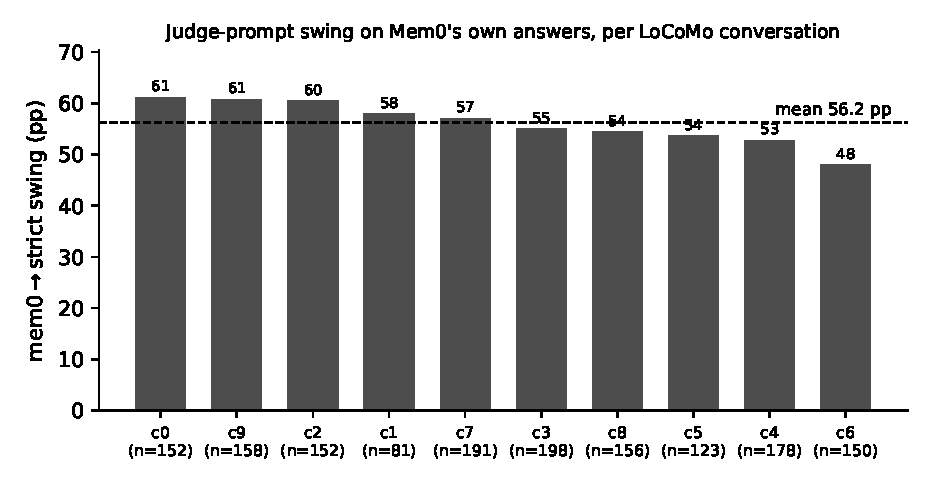
\includegraphics[width=0.74\linewidth]{../../figures/crossconv_swing.pdf}
\caption{The \texttt{mem0}$\to$\texttt{strict} swing on Mem0's \emph{own} published LoCoMo answers, per conversation ($n=1539$). The lenient prompt lands within 1.5 points of Mem0's reported 92.5\%; the strict prompt yields ${\sim}35\%$. The swing is 48--61 points in every conversation---universal, not specific to conv-26 (bar \texttt{c0}, the slice the control experiments use). Source: committed \texttt{experiments/hardening/summary.json}.}
\label{fig:crossconv}
\end{figure}

\textbf{Isolating prompt from model.} On our engine's fixed 152-answer conv-26 set, holding \texttt{gpt-5} fixed and changing the prompt moves the score from 0.9013 to 0.4803 (42.1 points); holding the Mem0 prompt fixed and changing the model to \texttt{gpt-4o} moves it to 0.9145 (1.3 points).\footnote{\path{kit/data/rejudge_20260521_235650.json}; all four judges grade the same answers.} The 1.3-point observed model contrast is of the same order as this judge's own repeat variability (implied sd $\approx$1.0 point at $n=152$; the $\approx$0.5--0.7-point figure of \S\ref{sec:threats} averages over four judges, two of which never varied across repeats), and that exact contrast was not itself repeated enough to establish a tail probability. The descriptive separation remains large: 1.3 observed points versus 42.1 under the prompt intervention. Across these 152 answers the strict judge never scores a question higher than the generous judge.

\textbf{The decomposition holds on the full run.} Extending the same two-axis decomposition to all 1{,}539 published answers:\footnote{\path{scripts/run_model_vs_prompt_fullset.py}; per-answer verdicts \path{experiments/hardening/verdicts/MV_conv*.json}; per-conversation table \path{experiments/hardening/model_vs_prompt_fullset.md}.} holding the model fixed, the prompt moves the run-level score by $+56.1$\,pp under \texttt{gpt-5} and $+48.8$\,pp under \texttt{gpt-4o}; holding the prompt fixed, the \texttt{gpt-5}$\,{-}\,$\texttt{gpt-4o} score difference is $-0.9$\,pp under the lenient prompt and $-8.2$\,pp under the strict one: \texttt{gpt-4o} is the \emph{more generous} backbone under both prompts, markedly so under the strict rubric. The $2\times2$ identity closes exactly---the difference between the two prompt effects ($56.1-48.8=+7.3$) equals the difference between the two model effects, $-0.9-(-8.2)$---and the artifact script asserts it. The prompt dominates on every conversation under both backbones (per-conversation prompt effect ranging from $+44.7$\,pp under \texttt{gpt-4o} to $+61.2$ under \texttt{gpt-5}; model effect, same \texttt{gpt-5}$\,{-}\,$\texttt{gpt-4o} convention, $-10.5$ to $+1.9$), with a mean absolute prompt effect of $52.4$\,pp against $4.5$ for the model---an order of magnitude: the full-run counterpart of the conv-26 extreme above, where the model effect was an order of magnitude smaller. The asymmetry is itself informative, and a third, non-OpenAI backbone sharpens it. Re-scored on \texttt{claude-sonnet-4-5}, the lenient prompt scores \textbf{91.9\%} and the strict prompt \textbf{62.8\%}.\footnote{\path{scripts/run_extra_judges.py}; verdicts \path{experiments/hardening/verdicts/XB_conv*.json}; summary \path{experiments/hardening/third_backbone.md}. Judges \texttt{mem0-claude}, \texttt{strict-claude}.} The \emph{lenient} endpoint is thus model-invariant to within one point across all three backbones (\texttt{gpt-5} 91.0, \texttt{gpt-4o} 91.9, Claude 91.9), whereas the \emph{strict} endpoint is strongly model-dependent (35.0 / 43.1 / 62.8): ``be strict'' is an instruction different models obey to different degrees. A distant backbone does narrow the swing---from 56 points on \texttt{gpt-5} to 29 on Claude---but through the strict endpoint alone; the field's lenient prompt, the one actually driving published headlines, is backbone-independent. A rubric's model-robustness is one more property an unpinned judge configuration silently varies.

\textbf{Which leniency rule carries the swing.} The lenient prompt bundles four tolerances---partial credit, paraphrase, date/duration windows, and acceptance of extra unverified detail about the same referent. Tightening each one alone to the strict standard, over the full run, isolates its contribution:\footnote{Four ablation prompts \path{kit/prompts/judge_abl_*.txt}, each the lenient prompt with exactly one rule replaced by its strict form; verdicts \path{experiments/hardening/verdicts/ABL_conv*.json}, summary \path{experiments/hardening/ablation.md}.} forbidding \emph{unverified extra detail / same-referent-different-fact} alone drops the lenient 91.0\% by \textbf{25.4}\,pp, far more than partial credit (7.1), date tolerance (4.3), or paraphrase (3.1) (each drop on the answers jointly scorable under that variant, $n=1381$--$1539$; the date-tolerance judge left 158 unparseable---its drop is bounded to $[3.3, 13.6]$\,pp under \emph{any} handling of those rows, counting them all-correct or all-wrong, and the extra-detail rule dominates under every handling; \path{scripts/ablation_unparseable_bounds.py}). Restricting to the single common denominator---the $n=1371$ answers jointly parseable under all six judges---changes nothing that matters: drops 25.6 / 6.8 / 4.1 / 3.2\,pp, same ordering, full swing 55.9 (\path{scripts/stats_ci.py}). The largest marginal single-rule effect is therefore not partial credit, as the multi-hop concentration might suggest, but the prompt's willingness to credit padded or loosely-attributed answers (full attribution would need a $2^4$ factorial, which we leave to the follow-up program). On that common denominator the four single-rule drops sum to 39.7\,pp against the full 55.9 swing. The direction of that 16-point residual is informative: mere overlap---one answer caught by several tightened rules---would make the sum \emph{exceed} the composite, since the answer is counted once per rule. The sum falling \emph{short} is therefore a non-additivity diagnostic pointing the other way: some answers survive every single tightening and flip only when the constraints tighten jointly, or the judge responds nonlinearly to the composite prompt. A one-factor-at-a-time design cannot separate those two, so we report the gap rather than identify the interaction---the composite prompt is more than its parts, and how much more needs the $2^4$ factorial named in \S\ref{sec:nextgen}.

% table_judge_swing.tex -- judge-swing decomposition. Deps: booktabs only.
% Wire with: % table_judge_swing.tex -- judge-swing decomposition. Deps: booktabs only.
% Wire with: % table_judge_swing.tex -- judge-swing decomposition. Deps: booktabs only.
% Wire with: \input{../../figures/table_judge_swing}
\begin{table}[t]
\centering
\caption{Accuracy of the \emph{same} 152-answer set (our engine's answers on
LoCoMo conv-26) as a function of the judge. Switching from the \texttt{mem0}
lenient prompt to the \texttt{strict} prompt while keeping \texttt{gpt-5} drops
the score by 42.1\,pp; swapping the model from \texttt{gpt-5} to \texttt{gpt-4o}
while keeping the \texttt{mem0} prompt moves it by only 1.3\,pp. The judge
\emph{prompt} dominates the judge \emph{model} as a source of score variance.}
\label{tab:judge-swing}
\small
\begin{tabular}{@{}lllrl@{}}
\toprule
Judge & Prompt & Model & Acc.\ (\%) & vs \texttt{mem0} \\
\midrule
\texttt{mem0}       & generous (partial, $\pm$14\,d)     & gpt-5      & 90.1 & --- \\
\texttt{mem0-4o}    & generous (partial, $\pm$14\,d)     & gpt-4o     & 91.5 & $+1.3$ \\
\texttt{mnemoverse} & binary (exact, no tolerance)         & gpt-5-mini & 75.7 & $-14.5$ \\
\texttt{strict}     & strict (no paraphrase, no tolerance) & gpt-5      & 48.0 & $-42.1$ \\
\midrule
\multicolumn{5}{@{}l}{\textit{Decomposition on the same 152 answers:}} \\[2pt]
\quad prompt swap & \texttt{mem0}$\to$\texttt{strict} & gpt-5 fixed     & & $-42.1$\,pp \\
\quad model swap  & gpt-5$\to$gpt-4o                  & \texttt{mem0} fixed & & $+1.3$\,pp \\
\bottomrule
\end{tabular}

\vspace{2pt}
{\footnotesize Raw fractions: 0.9013 / 0.9145 / 0.7566 / 0.4803; $n=152$ for all
judges; percentage-point deltas are computed from the raw fractions, not the
rounded Acc.\ values. The \texttt{mnemoverse} judge uses a distinct binary prompt
implementation (ASYM-004) and is excluded from the prompt-vs-model decomposition.}
\end{table}

\begin{table}[t]
\centering
\caption{Accuracy of the \emph{same} 152-answer set (our engine's answers on
LoCoMo conv-26) as a function of the judge. Switching from the \texttt{mem0}
lenient prompt to the \texttt{strict} prompt while keeping \texttt{gpt-5} drops
the score by 42.1\,pp; swapping the model from \texttt{gpt-5} to \texttt{gpt-4o}
while keeping the \texttt{mem0} prompt moves it by only 1.3\,pp. The judge
\emph{prompt} dominates the judge \emph{model} as a source of score variance.}
\label{tab:judge-swing}
\small
\begin{tabular}{@{}lllrl@{}}
\toprule
Judge & Prompt & Model & Acc.\ (\%) & vs \texttt{mem0} \\
\midrule
\texttt{mem0}       & generous (partial, $\pm$14\,d)     & gpt-5      & 90.1 & --- \\
\texttt{mem0-4o}    & generous (partial, $\pm$14\,d)     & gpt-4o     & 91.5 & $+1.3$ \\
\texttt{mnemoverse} & binary (exact, no tolerance)         & gpt-5-mini & 75.7 & $-14.5$ \\
\texttt{strict}     & strict (no paraphrase, no tolerance) & gpt-5      & 48.0 & $-42.1$ \\
\midrule
\multicolumn{5}{@{}l}{\textit{Decomposition on the same 152 answers:}} \\[2pt]
\quad prompt swap & \texttt{mem0}$\to$\texttt{strict} & gpt-5 fixed     & & $-42.1$\,pp \\
\quad model swap  & gpt-5$\to$gpt-4o                  & \texttt{mem0} fixed & & $+1.3$\,pp \\
\bottomrule
\end{tabular}

\vspace{2pt}
{\footnotesize Raw fractions: 0.9013 / 0.9145 / 0.7566 / 0.4803; $n=152$ for all
judges; percentage-point deltas are computed from the raw fractions, not the
rounded Acc.\ values. The \texttt{mnemoverse} judge uses a distinct binary prompt
implementation (ASYM-004) and is excluded from the prompt-vs-model decomposition.}
\end{table}

\begin{table}[t]
\centering
\caption{Accuracy of the \emph{same} 152-answer set (our engine's answers on
LoCoMo conv-26) as a function of the judge. Switching from the \texttt{mem0}
lenient prompt to the \texttt{strict} prompt while keeping \texttt{gpt-5} drops
the score by 42.1\,pp; swapping the model from \texttt{gpt-5} to \texttt{gpt-4o}
while keeping the \texttt{mem0} prompt moves it by only 1.3\,pp. The judge
\emph{prompt} dominates the judge \emph{model} as a source of score variance.}
\label{tab:judge-swing}
\small
\begin{tabular}{@{}lllrl@{}}
\toprule
Judge & Prompt & Model & Acc.\ (\%) & vs \texttt{mem0} \\
\midrule
\texttt{mem0}       & generous (partial, $\pm$14\,d)     & gpt-5      & 90.1 & --- \\
\texttt{mem0-4o}    & generous (partial, $\pm$14\,d)     & gpt-4o     & 91.5 & $+1.3$ \\
\texttt{mnemoverse} & binary (exact, no tolerance)         & gpt-5-mini & 75.7 & $-14.5$ \\
\texttt{strict}     & strict (no paraphrase, no tolerance) & gpt-5      & 48.0 & $-42.1$ \\
\midrule
\multicolumn{5}{@{}l}{\textit{Decomposition on the same 152 answers:}} \\[2pt]
\quad prompt swap & \texttt{mem0}$\to$\texttt{strict} & gpt-5 fixed     & & $-42.1$\,pp \\
\quad model swap  & gpt-5$\to$gpt-4o                  & \texttt{mem0} fixed & & $+1.3$\,pp \\
\bottomrule
\end{tabular}

\vspace{2pt}
{\footnotesize Raw fractions: 0.9013 / 0.9145 / 0.7566 / 0.4803; $n=152$ for all
judges; percentage-point deltas are computed from the raw fractions, not the
rounded Acc.\ values. The \texttt{mnemoverse} judge uses a distinct binary prompt
implementation (ASYM-004) and is excluded from the prompt-vs-model decomposition.}
\end{table}


\textbf{A two-point gap does not resolve on this slice.} Everything above holds the answers fixed and measures absolute score sensitivity; the standard defense of a shared judge is that it at least preserves system ranking. Our public matrix contains five answer pipelines on LoCoMo conv-26, with one reader, one reader prompt, 152 questions, and shared judge-prompt hashes (Table~\ref{tab:protocol} states what is and is not equalized). Across four judges, 2 of 10 observed pipeline pairs flip; a paired question bootstrap puts the central 95\% of the flip-count stability distribution at $[0,4]$.\footnote{Per-question verdicts: \path{kit/data/matrix_conv26_perq.json}. Analysis: \path{scripts/rank_bootstrap.py} $\to$ \path{experiments/hardening/rank_bootstrap.md}. This is a stability range under this observed question frame, not a coverage-established confidence interval.} Because the range includes zero, we do not claim that judges reorder memory systems in general. The result is limited to the resolution of margins on this slice.

The two observed flips are separated by 3 and 4 answers (2.0 and 2.6 points---several times the $\approx$0.5--0.7-point run-to-run noise of \S\ref{sec:threats}, measured on other runs; this matrix itself was not re-graded). Each survives only 66\% and 76\% of question resamples. Thus a margin of this size does not resolve on these 152 questions. We do not extend that statement to full-run leaderboards, whose effective sample sizes, paired discordances, and dependence structures differ; each leaderboard must report its own paired uncertainty. The 2026 headline gaps of similar numerical size (\S\ref{sec:survey}) motivate that check but are not adjudicated by this slice. The matrix winner differs across judges in 66.6\% of bootstrap resamples under a tie-aware rule, but two judges are ours and the result remains a single-conversation observation, not a general law.

\textbf{The harness is a channel too---and here, a larger one.} One number in Table~\ref{tab:rank-reversal} deserves to be read against Table~\ref{tab:perconv}, because a reader will otherwise find the gap and draw a conclusion worse than the truth warrants. Mem0's hosted platform scores \textbf{70.4\%} in our harness under the lenient prompt on conv-26---and \textbf{92.1\%} on the same conversation, under the same prompt, on its \emph{own} published answers (Table~\ref{tab:perconv}, row \texttt{conv 0}). Both numbers are correct under their own configurations, and the 22-point distance between them is not a claim about Mem0: it is the measure of everything our harness changes---our reader and its prompt, retrieval capped at $k=50$, ingestion through the vendor's public API on our schedule, and the asymmetries the inventory of \S\ref{sec:repro} enumerates. We state it plainly: \emph{a re-hosted system is not the same measurement as the vendor's own pipeline}. On this same conversation the calibrated judge puts the lenient prompt's inflation at $+6.6$ points (Table~\ref{tab:perconv}, row \texttt{conv 0}), so the harness channel here is roughly three times it---an uncontrolled composite against a paired estimate, indicative rather than a decomposition, and still well under the 56 points an undisclosed judge choice can move. Our own engine carries the identical discrepancy, and we name it rather than let the asymmetry stand: 90.1\% on the Table~\ref{tab:judge-swing} answer set against 0.770 in the matrix sweep---13 points, on the same conversation under the same lenient prompt, the difference again being reader and prompt rather than memory. Two implications follow. Our matrix numbers are not comparable to any vendor's published headline---or to our own reported numbers elsewhere in this paper---and we do not present them as such. And the whole harness configuration---reader, reader prompt, token budget, retrieval cap, ingestion schedule, API configuration---belongs in the measurement contract beside the judge prompt. This evidence does not license attributing the 22 points to reader budget or retrieval depth \emph{individually}: it is an uncontrolled composite, and all it shows is that the composite moved this score further than the field's realized judge choice did (and less far than the constructed 56-point prompt span).

We ran one further pipeline on this slice and keep it out of the table, deliberately. A naked-cosine baseline exists here too, and under the lenient prompts it outscores every pipeline in the matrix (0.809 and 0.882, against 0.579--0.789 and 0.658--0.822)---but it ran on our other runner path, whose answers average 105 characters against 43--70 for the harness pipelines. Since the single-rule ablation above measures the lenient prompt's tolerance for unverified extra detail at 25.4\,pp---the dominant lever---a lenient-judge win for the longest answers on the slice is confounded with answer format and cannot be read as evidence about memory. We name the finding we cannot yet make: whether a trivial baseline beats commercial memory under the field's judge, on a reader-symmetric run, is a question this matrix cannot settle and the follow-up program (\S\ref{sec:nextgen}) can.

\begin{table}[t]
\centering
\caption{What the conv-26 matrix does and does not equalize. All five pipelines ran in one harness sweep with one reader (\texttt{gpt-5-mini}), one reader prompt (no category hints on any row), one question set ($n=152$, the non-adversarial subset), and identical judge prompt hashes. What differs is what a memory system \emph{is}: hosted platforms embed and retrieve with their own internal representations, so ``same embeddings'' holds only for the pipelines that use ours. Depth is what the store actually returned, not what was requested. Retrieval depths recomputed from the harness cells' \texttt{retrieved\_atom\_ids}; transports from their \texttt{system\_config}. Those source cells sit in the private core checkout named in \texttt{kit/data/matrix\_conv26\_perq.json}'s provenance block, from which the per-question verdicts here were extracted.}
\label{tab:protocol}
\small
\begin{tabular}{@{}llll@{}}
\toprule
Pipeline & Transport & Embeddings & Median atoms returned at $k{=}50$ \\
\midrule
mnemoverse engine & in-process & \texttt{text-embedding-3-small} & 50 (up to 74; two-pass + reranker) \\
mnemoverse http   & our public API & internal & 60 (up to 75) \\
mem0 v3           & vendor API & vendor-internal & 50 \\
supermemory       & vendor API & vendor-internal & \textbf{7.5} (max 25) \\
zep               & vendor API & vendor-internal & 50 \\
\bottomrule
\end{tabular}

\vspace{2pt}
{\footnotesize The supermemory row is the largest disclosed asymmetry in the table and it runs \emph{against} that vendor: its API returned a median of 7.5 atoms where the others returned 50, so its scores are not a measurement of supermemory at depth 50. We report it rather than quietly drop the row.}
\end{table}

\begin{table}[t]
\centering
\caption{Five answer pipelines $\times$ four judges, LoCoMo conv-26 at $k=50$ (one harness sweep; judge-scored accuracy with answer counts, $n=152$). Two of the ten pairs change order between judges---\texttt{engine}\,/\,\texttt{supermemory} and \texttt{http}\,/\,\texttt{zep}---on margins of 3 and 4 answers (2.0 and 2.6 points---larger than the $\approx$0.5--0.7-point run-to-run noise seen in separate repeat studies, but fragile to which questions are asked: the paired bootstrap puts the central 95\% of the flip count at $[0,4]$), so we report this as an unstable ranking, not as a measured reversal. Two of the four judges (\texttt{strict}, \texttt{mnemoverse}) are ours. Recomputes offline: \texttt{scripts/rank\_bootstrap.py}.}
\label{tab:rank-reversal}
\small
\begin{tabular}{@{}lrrrr@{}}
\toprule
& \multicolumn{2}{c}{field-style lenient prompts} & \multicolumn{2}{c}{author-written prompts} \\
\cmidrule(lr){2-3}\cmidrule(lr){4-5}
Pipeline & \texttt{mem0} & \texttt{mem0-4o} & \texttt{strict} & \texttt{mnemoverse} \\
& \footnotesize gpt-5 & \footnotesize gpt-4o & \footnotesize gpt-5 & \footnotesize gpt-5-mini \\
\midrule
mem0 v3 (hosted)  & 0.704 (107) & 0.724 (110) & 0.270 (41) & 0.625 (95) \\
mnemoverse engine & 0.770 (117) & \textbf{0.822} (125) & \textbf{0.388} (59) & \textbf{0.711} (108) \\
mnemoverse http   & 0.579 (88)  & 0.658 (100) & 0.217 (33) & 0.408 (62) \\
supermemory       & \textbf{0.789} (120) & \textbf{0.822} (125) & 0.349 (53) & 0.651 (99) \\
zep               & 0.638 (97)  & 0.684 (104) & 0.191 (29) & 0.480 (73) \\
\bottomrule
\end{tabular}

\vspace{2pt}
{\footnotesize Bold marks each judge's top pipeline; \texttt{mem0-4o} ties engine and supermemory exactly (125 answers each), which the tie rule does not count as a flip. The lenient \texttt{mem0} prompt crowns supermemory; the other three crown our engine. Read the table for the instability of the ordering, never for the ordering.}
\end{table}

The consequence of the prompt swing is structural, not incidental. Across-paper comparisons made under different unpublished prompts confound grading policy with system behavior. Sharing one prompt removes that cross-paper degree of freedom, but it does not guarantee unbiased absolute scores or equal residual error across answer sets. In our vendor run the lenient-minus-calibrated sign is consistent across ten conversations; its magnitude is not established as uniform across systems. The field already describes such scores as approximate rankings\citep[\S5.3]{synthius} and notes, in a cost-estimate appendix, the absence of an independent identical-conditions audit.\citep[App.~A.5]{synthius} Our contribution is to measure the free rubric coordinate on fixed answers: a 56-point constructed stress span, a 10.3-point contrast between published rubrics on \texttt{gpt-4o} backbones, and a provisional 5.7-point contrast against \texttt{golden-v2}. Any comparison that does not pin prompt, model, and rubric leaves a large measurement coordinate free.

We stress what this result is \emph{not}. It is not a claim that any particular system is better or worse than another: the headline swings are each computed on a single fixed answer set, so no system is advantaged there, and the multi-judge matrix (Table~\ref{tab:rank-reversal}) is read only for the \emph{instability} of its ranking, never for the ranking itself. It is not a claim that LLM-as-judge is the wrong tool---\S\ref{sec:recall} argues it is necessary but must be paired with a judge-free floor. It is not a claim that the generous prompt is ``wrong'' and the strict prompt ``right.'' The point is precisely that the choice is currently free, undeclared, and decisive. The remedy we point to (\S\ref{sec:repro}, \S\ref{sec:nextgen}) is not a better prompt but a \emph{fixed, shared} one, reported alongside a metric the judge cannot inflate.

\section{Judging the judges}\label{sec:judges-error}

Section~\ref{sec:judge} shows the judges disagree by forty to fifty-six points but treats none of them as correct. The obvious next question is whether any of them \emph{is}: on a benchmark with reference answers, we can measure each judge's error against ground truth rather than against the other judges.

The difficulty is that ``ground truth'' for whether a free-text answer is correct is the very thing an LLM judge approximates---so we cannot use a judge to grade the judges. We use two standards. The first is a rule---a \emph{strict lexical-containment proxy}. An answer counts as correct if the normalized gold value appears in it as a substring, if every token of a multi-word gold appears somewhere in the answer, or if a date variant of the gold matches a date variant of the answer. The rule applies only to questions whose gold is a discrete value of at most eight tokens; relational golds such as ``the week before X'' are kept only when they carry a concrete date, and are matched on that date text without resolving the relation. On LoCoMo conversation~26 this rule-decidable subset is 117 of 152 questions. The exclusions are the open-domain questions and those whose gold is longer than eight tokens; no relative-date gold is excluded, since every one in this conversation carries a concrete date. Against the proxy, each judge makes two kinds of error: a \emph{false positive}---crediting an answer the proxy rejects (leniency)---and a \emph{false negative}---rejecting an answer the proxy accepts (strictness). One property of the proxy must be named before the table: the proxy is itself strict---it credits nothing the gold string does not license, no paraphrase, no partial recall---so it \emph{structurally favors strict-leaning judges}. Its verdict is a beginning, not the truth. The second standard is a blind human adjudication, below, which puts the proxy itself on trial.

\begin{table}[t]
\centering
\caption{Each judge's error against the strict lexical-containment \emph{proxy} on the rule-decidable subset of LoCoMo conv-26 ($n=117$), grading our engine's answers. FP (leniency) $=$ credited an answer the proxy rejects; FN (strictness) $=$ rejected an answer the proxy accepts. The proxy shares the strict prompt's strictness, so FP is a measure of leniency relative to the proxy (the proxy itself accepts wrong answers that contain the gold string, so its bias is two-sided), and this ranking is the \emph{proxy's}, not a human's: the blind human adjudications---of the control slice and of this table's own answer set (see text)---invert it.}
\label{tab:judge-error}
\small
\begin{tabular}{@{}llrrr@{}}
\toprule
Judge & Model & Acc.\ vs proxy & FP (leniency) & FN (strictness) \\
\midrule
\texttt{mem0}       & gpt-5      & 59.8\%          & 78.3\% & 0.0\% \\
\texttt{mem0-4o}    & gpt-4o     & 57.3\%          & 83.3\% & 0.0\% \\
\texttt{strict}     & gpt-5      & \textbf{74.4\%} & 28.3\% & 22.8\% \\
\texttt{mnemoverse} & gpt-5-mini & 70.1\%          & 53.3\% & 5.3\% \\
\bottomrule
\end{tabular}

\vspace{2pt}
{\footnotesize On the control slice's answers (110 rule-decidable of 143) the \texttt{mem0} judge's FP falls to 58.8\% and \texttt{strict}'s FN rises to 33.3\%: the same judges, different error rates per answer set. Per-category numbers: \path{kit/scripts/judge_error/} (committed \texttt{judge\_error\_results.json}). Every number in this table---and the control-slice note above---recomputes from committed artifacts alone via \path{kit/scripts/recompute_judge_error.py} (answers + per-judge verdict arrays + the verbatim proxy rule; no private dependency, no API key).}
\end{table}

The proxy's pattern is stark (Table~\ref{tab:judge-error}). The \texttt{mem0} judge---the field-standard prompt, the one on our own public benchmark page---never rejects a proxy-right answer (false-negative rate 0\%) yet credits 47 of 60 proxy-wrong answers (false-positive rate 78\%). The author-specified \texttt{strict} judge is, \emph{against the proxy}, the most accurate of the four judges (74\% versus 60\% for \texttt{mem0}); two of the four, \texttt{strict} and \texttt{mnemoverse}, are ours, and we name them rather than obscure that the proxy's best grader is one we built. This looks like the empirical answer to the objection that the strict prompt was built as a strawman---until the proxy itself is put on trial.

So we put it on trial. On the control slice (\S\ref{sec:judge}), the two prompts disagree on 57 of the 143 answers---every one a case where the lenient prompt credits and the strict prompt rejects. All 57 were blind-adjudicated by a human: the annotator saw only question, gold, and answer, with the machine verdicts hidden. (One scoping note that covers every human verdict in this paper: annotators judged answers against the benchmark's \emph{reference} answer, not against the source conversation, so a human label here is a reference-matching judgment---``human-accepted'' means accepted relative to the gold, and source-grounded truth was not adjudicated.) The result: \textbf{40} of the 57 are the \emph{strict} prompt falsely rejecting an answer a human accepts---paraphrases (``trans'' for a gold of ``transgender woman''), honest partial recall of a list, same-window date expressions---only \textbf{3} are human-labeled over-credit (the lenient prompt crediting an answer the human rejects), and \textbf{14} are genuinely ambiguous. Under \emph{every} resolution of the ambiguous cases, the proxy's ranking \emph{inverts}: on this answer set the lenient prompt is closer to the human reference-matching judgment than the strict one by 16 to 36 points of accuracy. The proxy crowned the strict judge because the two share a bias; a paraphrase-crediting human crowns the lenient one. Even the three human-labeled over-credit cases counsel humility: two of them are themselves borderline calls. And the same adjudication on the engine-answer side of Table~\ref{tab:judge-error}---all 64 lenient-credits/strict-rejects disagreements on that answer set---is starker still: \textbf{57} are the strict prompt falsely rejecting a human-accepted answer, \textbf{zero} are human-labeled over-credits, and 7 are ambiguous (near-miss partial lists). Across both answer sets, 97 of 121 adjudicated disagreements are strict false rejections; three are human-labeled over-credits. Two further hypothesis-blind annotators---one now a co-author, one external to the work---reproduce the direction, crediting 100 and 93 of 121 against the strict prompt; the pre-specified three-rater majority is \textbf{102 of 121} strict false rejections against \textbf{1} human-labeled over-credit (\S\ref{sec:threats}).\footnote{The adjudication covers all 57 control-slice and all 64 engine-side lenient/strict disagreements; integrity checks confirm every labeled case is a genuine disagreement with the recorded direction. The primary annotator is the lead author---disclosed, and blind to machine verdicts; labels ship at \path{kit/judge_audit/}. An out-of-sample validation set is reported below; the relabeling campaign and its reconciliation are reported in \S\ref{sec:threats}, with all labels and the pre-specified analysis at \path{kit/annotation/}. Details: \path{kit/docs/PROVENANCE_NOTES.md}, P6.}

The two verdicts together are the finding. Against a strict rule, the strict prompt wins; against a blind human, the lenient prompt wins---\emph{on naturally produced, mostly honest answers}. Neither statement makes either prompt a good judge. The lenient prompt's written rules remain mechanically exploitable: its partial-credit rule is obliged to credit an answer that lists several mutually exclusive candidates, one of which happens to be right---a pattern that actually occurs in the control slice---and an independent public audit reports that a generous LoCoMo judge configuration accepted 62.81\% of deliberately vague-but-topical wrong answers\citep{locomoaudit}. The strict prompt, symmetrically, rejects the large majority of correct paraphrases a human accepts. Which judge is ``most accurate'' is an artifact of the truth-standard chosen to measure it. (One shared caveat sits under every accuracy figure in this section, human included: the benchmark's own answer key carries errors---a reported 6.4\% error rate in one independent grey-literature audit\citep{locomoaudit}---so some fraction of every grader's verdicts, human included, is scored against a wrong gold.)

A second finding is robust across both truth-standards we applied. The same judge errs by different amounts depending on whose answers it grades: against the proxy, the \texttt{mem0} judge's false-positive rate is 78\% on our engine's answers but 59\% on the Mem0-backed control slice's answers---a nineteen-point difference, on answer sets that share our reader, so the difference isolates the memory path with the reader held constant. The two sets also share their \emph{questions}---they are two systems' answers to the same conv-26 items---so we test the difference in a way that respects that: a cluster bootstrap over the shared question frame puts it at $+17.9$\,pp, 95\% interval $[+4.4, +31.7]$, negative in 0.5\% of resamples.\footnote{\path{scripts/differential_error_paired.py}, which reuses the proxy rule and the rule-decidable filter verbatim from \path{kit/scripts/judge_error/compute_judge_error.py}. This supersedes the two-proportion test earlier versions of this paper reported ($p \approx 0.02$): that test assumes independent samples, and two systems answering the same questions are not independent. The clustered result is the one we stand behind.}

On the 110 jointly rule-decidable questions, the aggregate error gap can be localized but not mechanistically explained. On the 46 questions where both systems are proxy-wrong, the judge credits 34 answers from each ($p=1.0$ under the paired label permutation). The aggregate gap lies in different singleton-wrong question sets: 9 of 10 engine-only errors are credited versus 6 of 22 control-only errors. Because these strata contain different questions, potentially with different difficulty and error types, the result establishes answer-set composition dependence, not a system--judge interaction or differential treatment of matched failures. A blinded error-type annotation or crossed-answer design is required for the stronger claim and is part of the follow-up program.

\textbf{A constructive step: a human-calibrated judge.} The adjudication above is not only an indictment; it is a calibration target. From the failure taxonomy of the adjudicated disagreements---paraphrase, honest partial recall, and same-window dates on the credit side; multi-candidate hedging, pseudo-item padding, and vagueness on the integrity side---we specified a new grading prompt, \texttt{golden} (v2, shipped in the kit), that credits meaning while refusing the known exploits, on the same \texttt{gpt-5} backbone as the other judges. We then validated it \emph{out of sample}: 54 answers drawn from nine conversations never used in its calibration, blind-labeled by the annotator \emph{after} the judge's verdicts had been computed and sealed. (The 54 are sampled---seeded, stratified, six per conversation---from the same vendor-published Platform run the judge is applied to below, so the validation measures transfer to exactly the answer style it is later asked to grade.) It agrees with the human on 43 of the 44 decided cases (97.7\%; Wilson 95\% CI $[88.2\%, 99.6\%]$; the annotator marked 10 of the 54 ambiguous, so decided-case coverage is 44/54), with zero over-credits and one over-rejection; the field's lenient prompt agrees on 41 (93.2\%; all three misses are over-credits), and the naive strict prompt on 24 (54.5\%; twenty over-rejections). Table~\ref{tab:val54} assembles every grader on these same 54 answers against every human standard, including the two raters who never saw any rubric under test and the three-rater majority. The ambiguity rate itself---7.4\% to 18.5\% of the 54, depending on the rater---is not a nuisance statistic but part of this paper's finding: the human rubric, too, is soft at the boundary, and where a rater draws that boundary moves the band they imply. At this $n$ the calibrated and lenient agreement rates are not statistically separable; what separates them is the error \emph{character}---the calibrated judge's single miss is an over-rejection, the lenient prompt's three are all over-credits---and the band placement below. The error character also bounds the direction of any residual bias, conditionally: \emph{if} the validation-observed error direction generalizes to the full run, residual calibrated-judge error biases the inflation estimate upward, not downward (one observed miss cannot rule out unseen over-credits; the conditional is the honest form). On the validation slice the lenient prompt exceeds even the most generous resolution of the human labels---but by one answer of 54 (Table~\ref{tab:val54}), so we report it as a one-answer exceedance of the observed rater-implied bands, not as a judge-independent bound: one changed decided label erases it. On the same 54 answers the lead annotator's labels imply a score in $[70.4\%, 88.9\%]$ (the width is the ambiguous cases); the calibrated judge scores 85.2\%---inside it---while the lenient prompt scores 94.4\%, above even the generous end. That comparison uses the annotator who wrote the calibrated rubric, so we repeat it against the two who did not: their bands sit higher and narrower ($[83.3, 92.6]$ and $[85.2, 92.6]$; three-rater majority $[83.3, 92.6]$), and the lenient prompt's 94.4\% remains above all of them---by 1.8 points rather than 5.5. The direction survives every standard we have; the margin is smaller than the lead annotator's band alone would suggest, and we report both. (This 85.2\% is the 54-answer validation slice; the full-run 85.3\% below is a separate measurement over all 1{,}534 jointly-scored answers---numerically close by coincidence, not by construction.)

\begin{table}[t]
\centering
\caption{Every grader on the \emph{same} 54 validation answers, against every human standard. \emph{Implied band} is the score range a standard permits, from resolving its ambiguous cases all-wrong to all-correct; agreement is counted only on the cases that standard decides. The two additional raters never saw any rubric under test. LongMemEval is scored here on the same 54 items---the only denominator on which it is comparable to a band. Recomputes offline: \texttt{scripts/validation\_54\_all\_judges.py}.}
\label{tab:val54}
\small

\begin{tabular}{@{}lccc@{}}
\toprule
\multicolumn{4}{@{}l}{\emph{Human standards}} \\
\midrule
standard & correct / wrong / ambiguous & ambiguity rate & implied band \\
\midrule
lead annotator (E.\,I.) & 38 / 6 / 10 & 18.5\% & $[70.4, 88.9]$ \\
O.\,T.                  & 45 / 4 / 5  & 9.3\%  & $[83.3, 92.6]$ \\
A.\,S.                  & 46 / 4 / 4  & 7.4\%  & $[85.2, 92.6]$ \\
three-rater majority    & 45 / 4 / 5  & 9.3\%  & $[83.3, 92.6]$ \\
\bottomrule
\end{tabular}

\vspace{6pt}

\begin{tabular}{@{}lrrrrr@{}}
\toprule
\multicolumn{6}{@{}l}{\emph{Graders}: score on the 54, then agreement on each standard's decided cases} \\
\midrule
grader & score & lead (44) & O.\,T.\ (49) & A.\,S.\ (50) & majority (49) \\
\midrule
calibrated (\texttt{golden}) & 85.2\% & 43/44 & 46/49 & 47/50 & 47/49 \\
lenient (\texttt{mem0})      & 94.4\% & 41/44 & 47/49 & 48/50 & 48/49 \\
strict                       & 33.3\% & 24/44 & 21/49 & 22/50 & 22/49 \\
LongMemEval                  & 83.3\% & 38/44 & 44/49 & 43/50 & 44/49 \\
\bottomrule
\end{tabular}

\vspace{3pt}
{\footnotesize Read this table against our own interest. On \emph{agreement counts} the lenient prompt matches the two independent raters at least as often as the calibrated judge does (48/49 vs.\ 47/49 on the majority standard): at $n{\approx}49$ the two are inseparable, and the calibrated judge's advantage over the lenient prompt exists only against the annotator who wrote its rubric. Two things do separate them. The \emph{direction} of the misses: the lenient prompt's are over-credits; the calibrated judge's single miss against the lead annotator is an over-rejection, and against each additional rater it misses three times, once by over-credit and twice by over-rejection. And the \emph{aggregate}: the lenient 94.4\% sits above the top of every band above---including the two raters who credit most freely (92.6)---so on this slice the field's prompt scores higher than any resolution of any rater's labels permits. That is the load-bearing fact, and it is weaker than the lead annotator's band alone suggests: 1.8 points of margin, not 5.5---\emph{one answer of 54} (51 credited against a band top of 50), and the same answer as the lenient prompt's single decided-case miss against the majority. The 54-answer slice is therefore not what carries the inflation estimate; the full-run comparison against the calibrated judge is (\S\ref{sec:judges-error}), with this slice as the check that the calibrated judge is not itself out of human range. The calibrated 85.2\% and LongMemEval's 83.3\% sit inside the lead annotator's band; against the higher-banded raters the calibrated judge sits at their floor and LongMemEval just below it---i.e.\ if anything it scores answers too harshly, which would make the reported inflation an \emph{over}-estimate, the same direction \S\ref{sec:judges-error} names.}
\end{table}

On the vendor's full run, \texttt{golden-v2} scores 85.3\% against the lenient prompt's 91.0\%, a \textbf{5.7-point plug-in estimate} on the 1{,}534 jointly scored answers. Item and conversation-resampling intervals are $[4.6,6.9]$ and $[4.9,6.5]$, conditional on the committed \texttt{golden-v2} verdicts; they quantify sampling stability within the observed frames, not calibration, label, or superpopulation uncertainty.\footnote{\path{experiments/golden_judge/FULLRUN_GOLDEN_RESULTS.json}; \path{scripts/stats_ci.py}. Robustness, all recomputed by \path{scripts/per_conv_calibrated.py}: the estimate is 5.7--6.0 under every handling of the five calibrated-unparseable answers, and 5.6--5.7 with conversation 26---the calibration-adjacent one---excluded entirely; the per-conversation range is 3.3--8.6 (Table~\ref{tab:perconv}).} The sign is positive in each of the ten vendor conversations, but neither that fact nor the 54-item validation makes 5.7 a human-labeled full-run inflation estimate. The independent LongMemEval contrast corroborates direction, not magnitude. On our engine's conv-26 answers, \texttt{golden-v2} scores 79.5\% against the lenient prompt's 90.1\% on the 151 jointly-parseable answers---an analogous contrast of 10.6 points, nearly twice the vendor's, so the field's prompt flatters our own system more than the competitor's.\footnote{\path{experiments/golden_judge/verdicts_golden2_engine_conv26.json}; both operands on the jointly-parseable answers, the joint-denominator convention of Table~\ref{tab:perconv}.} Because the answer sets and their error composition differ, that demonstrates composition dependence rather than a system--judge interaction. \texttt{golden-v2} remains a useful model-based reference, not a fixed human truth standard: it was calibrated by one author and validated on 54 items, and would require independent multi-rater calibration at larger scale before benchmark adoption. What it is not is fitted to its own test: the v1$\to$v2 iteration used only the first adjudication---the control slice's 57 disagreements---as its calibration signal; the validation set was untouched during design, and its verdicts were computed and sealed before the validation labels existed. That ordering is the one prospective lock in this paper, and a reader can check it: the prompt, the sealed verdicts, and the labels ship separately.\footnote{Prompt: \path{kit/prompts/judge_golden_v2.txt}. Sealed verdicts: \path{experiments/golden_judge/verdicts_golden2_validation_set.json}; held-back comparison: \path{experiments/golden_judge/VALIDATION_RESULTS.json}; labels: \path{kit/judge_audit/human_labels_validation_set.json}.}

\begin{table}[t]
\centering
\caption{Per-conversation scores on Mem0's full published run: the field's lenient prompt vs.\ the human-calibrated judge (\texttt{golden} in artifact paths; same \texttt{gpt-5} backbone, same answers). Row \texttt{conv 0} is LoCoMo conv-26; Figure~\ref{fig:crossconv}'s axis labels c0--c9 use the same indexing. Jointly-scored answers; recomputes offline from committed per-answer verdicts via \texttt{scripts/per\_conv\_calibrated.py} (no API). Inflation is positive in all ten conversations.}
\label{tab:perconv}
\small
\begin{tabular}{lrrrr}
\toprule
conv & $n$ & lenient \% & calibrated \% & inflation (pp) \\
\midrule
0 & 151 & 92.1 & 85.4 & $+6.6$ \\
1 & 81  & 86.4 & 77.8 & $+8.6$ \\
2 & 152 & 96.1 & 91.4 & $+4.6$ \\
3 & 196 & 85.2 & 78.6 & $+6.6$ \\
4 & 177 & 87.0 & 80.2 & $+6.8$ \\
5 & 123 & 89.4 & 86.2 & $+3.3$ \\
6 & 150 & 92.0 & 86.7 & $+5.3$ \\
7 & 191 & 95.3 & 91.1 & $+4.2$ \\
8 & 156 & 91.7 & 85.9 & $+5.8$ \\
9 & 157 & 93.6 & 87.3 & $+6.4$ \\
\midrule
all & 1534 & 91.0 & 85.3 & $+5.7$ \\
\bottomrule
\end{tabular}

\vspace{2pt}
{\footnotesize The largest inflation (conv~1, $+8.6$) is also the smallest sample ($n=81$); the floor is $+3.3$ (conv~5). Five of the 1{,}539 answers are calibrated-unparseable and excluded from the joint denominator (listed by identifier in \path{scripts/per_conv_calibrated_output.md}). Inflation is computed at full precision before rounding, so a row may differ from the subtraction of its rounded columns by 0.1; robustness under every handling is 5.7--6.0\,pp.}
\end{table}

We do not claim a universally correct judge exists: the best judge under one standard is among the worst under another, and every judge in our set errs by different amounts on different systems. But the constructive result narrows the despair---a judge calibrated against a few dozen human adjudications lands within the human band on data it never saw (at its floor under the strictest-banded rater). What this section establishes is, we think, enough to unsettle current practice. The judge is not a neutral instrument that reads off a system's quality. It is a biased one, biased differently on different answer sets and differently under different truth-standards---and left unpinned, it can dominate the headline. The judge of the judges, it turns out, is also the benchmark.

\section{What the judge measures, and what it hides}\label{sec:recall}

\begin{figure}[t]
\centering
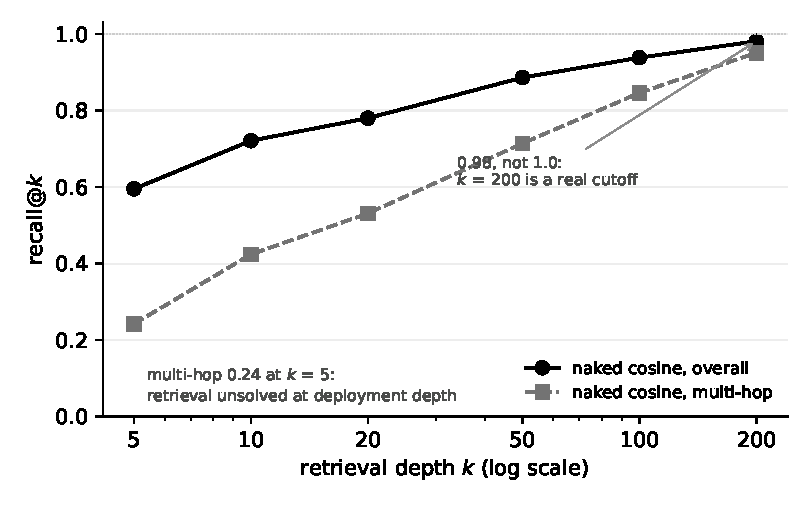
\includegraphics[width=0.64\linewidth]{../../figures/recall_k_curve.pdf}
\caption{Naked-cosine recall@$k$ on LoCoMo conv-26 ($n=150$ of the slice's 152 questions; two carry no evidence annotation), the saturation calibrator (recall certified \texttt{exact} by \texttt{recompute\_recall.py}). At large $k$ a trivial baseline retrieves the gold evidence nearly completely, so the headline's gap there is conversion, not retrieval; at small $k$, retrieval is genuinely hard (multi-hop 0.24 at $k=5$). Recall at $k=200$ is 0.98, not 1.0; the store holds 419 dialog-turn atoms, so $k=200$ covers 47.7\% of it---a real cutoff, not the whole memory.}
\label{fig:recall}
\end{figure}

If a judge can be removed as the sole arbiter of a headline number, what lies underneath it? We argue for a metric the judge cannot touch: \textbf{retrieval recall at k}---the fraction of a question's gold-evidence items that appear among the system's top-k retrieved memories. It requires no language model to compute. It is reconstructed offline by intersecting the identifiers of the retrieved memories with the benchmark's own gold-evidence annotations.\footnote{\path{kit/scripts/recompute_recall.py}---intersects a question's retrieved memory identifiers with its LoCoMo gold-evidence ids, aggregated per category; no LLM in the path.} A system either surfaced the evidence or it did not. No grading prompt can change that.

A judge-free metric is only honest if the system never had privileged access to what it is being scored on. Two rules make recall meaningful. First, an \textbf{anti-cheat constraint}: the retrieval query must contain only what a user would actually type---the question text---and never the gold-evidence identifiers, the category label, or the reference answer---and the same prohibition covers the \emph{reader} prompt that turns retrieved memories into the judged answer, because the generation stage is a channel worth tens of points (\S\ref{sec:judge}); our own control slice's disclosed legacy category hint (\S\ref{sec:judge}) is exactly this class of leak, which is why the constraint must bind the whole answer path. A benchmark that lets any of these reach the retriever or the reader is measuring oracle lookup, not memory. Second, \textbf{declared ingest compute}, best structured as two evaluation tracks. Write $\mu$ for the number of language-model calls a system makes while ingesting the conversation. A \emph{zero-LLM-ingest} track ($\mu = 0$, mechanically asserted) compares retrieval-only architectures. A \emph{declared-ingest-compute} track admits LLM-based extraction and consolidation---the interesting memory systems do this legitimately---but pins and publishes the ingest model, prompts, call and token counts, and cost, and asserts the ingest process had no access to the benchmark's questions. The integrity constraint targets \emph{gold leakage and undeclared precomputation}, not consolidation itself: a benchmark that only admits $\mu=0$ systems would architecturally exclude exactly the systems long histories require.\footnote{\path{kit/scripts/anti_cheat_audit.py} (scans the answer path for \texttt{qa.evidence}, \texttt{qa.category}, \texttt{qa.answer} --- the reference answer --- \texttt{adversarial\_answer}, and gold ids) and the integrity rules of \path{kit/docs/beam_integrity.md} (the $\mu = 0$ assertion: \texttt{llm\_calls\_during\_ingest == 0}, run aborts otherwise).} Both are mechanically checkable for systems run in-harness: the first by scanning the answer path for forbidden fields, the second by asserting the ingest LLM-call count (zero on the $\mu=0$ track, as-declared on the other). We call the first an \emph{automated leakage audit} rather than ``anti-cheat by construction'': a scanner over known field names catches accidental leakage, which is the common failure; it does not make deliberate circumvention impossible, and claiming so would be the kind of overstatement this paper is against. For hosted platforms that ingest server-side the counter is unobservable and any value is self-reported; such systems must run through declared network-intercepting instrumentation or be excluded from $\mu$-dependent claims. With that scope stated, both checks belong in the benchmark, not in the honor system.

With recall in hand, a simple diagnostic reframes the enterprise. We run a deliberately trivial baseline---\emph{naked cosine}: embed each memory, store the vectors, retrieve the top-$k$ by cosine similarity, with no learned structure, no consolidation, no reranking. On the conversation-26 slice of LoCoMo (150 of its 152 questions carry evidence annotations) its recall climbs from \textbf{0.60 at k = 5} through \textbf{0.94 at k = 100} to \textbf{0.98 at k = 200} (Figure~\ref{fig:recall}).\footnote{\path{kit/data/RECALL_AT_K_SUMMARY.json}; \path{kit/scripts/recompute_recall.py} recomputes the naked-cosine floor bit-for-bit and certifies it \texttt{exact}, but flags the learned engine's recall \texttt{n\_a}---consolidated atoms lack a guaranteed one-to-one map to gold-evidence ids---so we anchor on the naked floor and cite no engine-versus-naked delta. Both systems embed with \texttt{text-embedding-3-small}. Full curve: \path{kit/docs/PROVENANCE_NOTES.md}, P4.} Two consequences follow, and they cut in opposite directions. At large $k$, missing-evidence recall is nearly saturated \emph{for this retriever on this conversation}: the gold evidence is nearly always in the retrieved set. What then separates systems at that operating point is not failure to surface the evidence---it is everything downstream of surfacing it: distractor load and evidence precision in a 200-item context, context construction and ordering, the reader's ability to use evidence that is present, answer phrasing, and grading. We compress that bundle as \emph{conversion}, and note it is a bundle: recall saturation localizes the headline's variance downstream of evidence presence, not to any single stage---and saturation for the trivial baseline does not imply every system's retrieval is saturated. At small $k$---the low-depth operating points deployments favor---retrieval is not solved at all: naked-cosine multi-hop recall is \textbf{0.24 at k = 5}, so there the headline gap is partly a genuine retrieval failure. The single headline number therefore fuses, on this conversation and embedder, \emph{two} distinct failure modes---hard retrieval at low $k$ and lossy conversion at high $k$---and reports their blend as one ``memory'' score. We anchor this on the naked baseline, whose recall our tooling certifies as exactly reconstructable. A learned engine that consolidates memories need not preserve a one-to-one map from a retrieved atom to a gold-evidence id, so its own recall is not reconstructable to the same standard---a limitation we disclose rather than work around, and a reason to read any engine-versus-baseline recall comparison with caution. And k = 200 is a real cutoff, not simply the whole memory: the conv-26 store holds 419 dialog-turn atoms, so the top-200 covers just under half of it, and recall there is 0.98, not 1.0, and still climbing.

This is why we report recall first and the judge accuracy beside it, never in its place. Recall@k answers the question a memory benchmark is supposed to ask---\emph{did the system surface the right evidence?}---and answers it without a judge. The judge-mediated score answers a different, reader-dependent question and should be read as such. A benchmark that reports only the judge number leaves the two failure modes fused. At the high $k$ where retrieval is near-complete, it is in effect grading the language model that writes the final answer rather than the memory that found the evidence.

Our recall@$k$ metric provides judge-free grounding on the \emph{retrieval} axis: whether the memory system surfaced the evidence at all, independent of any grading model. A complementary axis is memory \emph{update}: Memora \citep{uddin2026memora} introduces Forgetting-Aware Memory Accuracy (FAMA), which penalizes reliance on obsolete or invalidated memories in long-horizon personalized-agent conversations. We note, however, that FAMA is itself judge-mediated---its per-criterion decisions are majority votes of a three-LLM judge panel---and therefore inherits the judge-configuration sensitivity we quantify here, albeit with model-level noise dampened by ensembling; the shared rubric, the coordinate our decomposition finds dominant (\S\ref{sec:judge}), is a single free variable that voting cannot average away. Extending judge-free measurement from the retrieval axis to the update/forgetting axis---a deterministic analogue of FAMA over labeled valid and invalidated memory traces---is a natural direction for future work.

\section{Reproducibility as a property of the benchmark, not the user}\label{sec:repro}

A fixed judge (\S\ref{sec:judge}) and a judge-free floor (\S\ref{sec:recall}) make a single measurement honest. They do not yet make two measurements comparable. The rest of the configuration still drifts: the engine changes between runs, the dataset is silently subsetted, the embedding model is swapped, the harness is rewritten. The field's own diagnosis---``no independent audit has measured all systems under identical conditions''\citep{synthius}---is a statement about configuration drift, and it cannot be answered by a better prompt. It is answered by treating reproducibility as a property the benchmark enforces, not a courtesy the practitioner extends. We propose three mechanisms. The first two are mechanically checkable in principle and are stated here as requirements a benchmark should enforce, not as machinery we ship; the third we do maintain, by hand.

\textbf{Version-pinned baselines.} A result carries an artifact-identity tuple: engine, harness, prospectively locked protocol, dataset hash, prompt hash, embedding model, reader and token budget, requested retrieval depth, evaluated evidence cutoff, and a resolved judge snapshot where available. For mutable provider aliases the tuple instead records alias, run timestamp, parser version, and verdict-artifact hash; such a result is artifact-frozen, not guaranteed rerun-identical. A coordinate change creates a new result identity rather than silently replacing the old one.

\textbf{A prospective provenance chain.} Before execution, the protocol, prompts, thresholds, parser, missing-verdict policy, and analysis plan are committed and timestamped as a lock; the run identifier binds that lock before raw results exist. Every public number then resolves to the locked protocol, immutable raw result, analysis output, registry entry, and artifact commit. Any rule change creates a new protocol version and run.\footnote{\path{kit/docs/provenance.md}; the claim-to-command registry and current execution surface are in \path{REPRODUCING.md}.} A figure that cannot be walked back along this chain is not citable. We have walked it manually across our own surfaces and retired or repaired the figures that did not resolve; the automated gate that would enforce it is specified here, not shipped. And the honest test of the discipline is what caught its failures: not us. External review caught our first frozen-manifest pin pointing to a commit that could not contain the artifact it named---the rule broke on its first application---after which we split source and artifact identity and recorded the failure rather than quietly repairing it. That is the argument of this paper turned on its author: self-applied integrity discipline is worth something, and it is not worth what an outside check is worth.

\textbf{Disclosed measurement asymmetries.} One cannot make heterogeneous systems identical---an in-process engine and a competitor reached only over HTTP do not run under the same conditions---but one can enumerate every way they differ and publish the list. We maintain a measurement-asymmetry inventory: a catalog of every advantage and disadvantage in the evaluation path, each classified by the side it favors.\footnote{\path{kit/docs/asymmetry_inventory.md}: 30 findings (ASYM-001..030); on current runs 16 favor Mnemoverse, 1 favors a competitor, the rest are two-sided, undetermined, or closed. Reconciliation of the two count breakdowns: \path{kit/docs/PROVENANCE_NOTES.md}, P7.} In our own setup it currently holds thirty findings, sixteen of which favor our own system; all are disclosed. This is the operational form of the honesty posture. A vendor that benchmarks itself cannot eliminate its conflict of interest, but it can convert that conflict into an auditable artifact and let the reader discount accordingly. This is also the concrete answer to the ``identical conditions'' gap: conditions are never identical, so the obligation is not to claim they are, but to make every non-identical condition visible.

None of the three mechanisms requires trusting the party that reports the number---which is the point. A benchmark whose integrity depends on the good faith of the vendors competing on it has none; these mechanisms move the guarantee into the artifact and the gate.

\section{Scale is necessary, and not sufficient}\label{sec:scale}

The most consequential recent move in this family is the jump in scale. BEAM\citep{beam} evaluates memory over single conversations of 100K, 500K, 1M, and 10M tokens. Nine of its ten abilities are scored by a nugget rubric: the reference answer is decomposed into atomic claims and the judge awards credit per claim. The tenth, event ordering, is scored by Kendall's $\tau_b$ after an LLM aligns events. The direction is right. Memory systems are built for histories spanning months or years, and a benchmark whose conversations span a handful of sessions---LoCoMo's regime---tests the wrong scale.\citep[\S5.4]{synthius} At ten million tokens the conversation exceeds the context windows of the models BEAM evaluates, so the memory engine becomes load-bearing in a way it never is at LoCoMo scale.

Scale does not repair the integrity problems of the preceding sections; it reproduces them at greater cost. BEAM's headline is still a judge-mediated score, and the published BEAM numbers already show the characteristic softness: the same vendor's public pages have carried two different BEAM-10M average-score values---48.6 and 45.0---with the aggregation method unspecified and no note reconciling them.\footnote{Both values are documented with sources in \path{kit/docs/competitor_claims.md}. Without dated archival snapshots and a specified aggregation we do not claim a temporal regression---only that the same benchmark's headline appears as two different numbers on the same vendor's surfaces, which is precisely the un-pinned-configuration failure \S\ref{sec:repro} addresses. We also run the paired-prompt intervention directly at this scale (below), so the softness is measured, not inferred.} The nugget rubric, moreover, awards partial credit for plausible phrasing, so a system can post a high pass-rate while its retrieval surfaced only a fraction of the gold evidence---the \S\ref{sec:recall} retrieval-versus-answer gap, now at the scale where it is most expensive to detect. The headline also depends on the reader as much as on the memory: how many tokens the engine feeds the reader is itself a free variable, so two BEAM numbers computed under different reader budgets are not comparable.\footnote{Reader-input token budget as a free variable: \path{kit/docs/beam_integrity.md} (the dual-track reader strategy and the \texttt{comparable: false} annotation across reader configurations).}

The prompt sensitivity of \S\ref{sec:judge} is not a LoCoMo artifact; it reappears at scale. We take our engine's answers to the 200 BEAM-10M questions and re-score them under the \emph{same} two prompts (the nugget rubric as the reference answer)---a stress-test of the rubric's prompt sensitivity, not a BEAM leaderboard entry: the lenient prompt scores \textbf{74.1\%}, the strict prompt \textbf{7.6\%}---a \textbf{66.5-point} swing on a fixed set of answers, larger than LoCoMo's 56, positive in every question type (from $+35$ on multi-session reasoning to $+100$ on summarization). The strict endpoint is especially low because most BEAM rubrics are multi-nugget, so the strict prompt's ``cover every item'' rule bites hard---the \S\ref{sec:judge} partial-credit finding again. But benchmark, answer set, and reference granularity all change together here, so the 66.5 points are a stress test on this answer set, not a measurement of scale itself.\footnote{Answers committed at \path{kit/data/beam_answers_10m.json} (extracted from a 10M-token engine run); runner \path{scripts/run_beam_rescore.py}; verdicts \path{experiments/hardening/verdicts/BEAM_*.json}; summary \path{experiments/hardening/beam_rescore.md}. $n=197$ of 200 jointly scored.} Scale multiplies the tokens; it does not pin the judge.

Scale is necessary, and a serious benchmark must adopt it. But a million-token benchmark with an unpinned judge, a pass-rate that outruns grounding, and an undeclared reader budget is the soft LoCoMo number with three more zeroes. Scale must arrive together with the \S\ref{sec:judge}--\S\ref{sec:repro} contract, or it merely raises the price of the same illusion.

\section{Toward trustworthy next-generation benchmarks}\label{sec:nextgen}

We can now state what a next-generation persistent-memory benchmark must provide. The requirements are deliberately about \emph{integrity}, not \emph{breadth}. They make a score trustworthy rather than adding more things to score.

\begin{enumerate}
  \item \textbf{A fixed, shared judge protocol}---one grading prompt, one model, one rubric, published and versioned, that every paper reporting on the benchmark must use. \S\ref{sec:judge} shows the alternative is a leaderboard that ranks prompts. Pinning the judge removes the free variable but does not equalize the judge's residual error across systems (\S\ref{sec:judges-error}); that residual is why item 2 must accompany this one.
  \item \textbf{A judge-free grounding metric, reported first}---recall of the gold evidence at $k$, reconstructed from identifiers without a language model, with any judge score reported beside it, never in its place (\S\ref{sec:recall}). One design obligation comes with it: identifier-level recall is only well-defined for stores that preserve atom-level identity, and a consolidating or abstracting memory---the interesting kind---need not. The benchmark, not the contestant, must close that gap: accept provenance-carrying consolidation (derived atoms citing their source identifiers), or score evidence coverage by span matching against the gold text, or provide a benchmark-side alignment pass. A grounding metric that only verbatim stores can report would penalize exactly the systems long histories require. This requirement currently binds only the \emph{retrieval} axis; a deterministic, judge-free analogue of FAMA \citep{uddin2026memora} would extend it to the update/forgetting axis (\S\ref{sec:recall} names the same gap on the answer side).
  \item \textbf{An automated leakage audit, and declared ingest compute}---gold evidence, category labels, and reference answers forbidden in the retrieval query and the reader prompt, mechanically scanned; ingest LLM usage either zero ($\mu=0$ track) or pinned and published (declared track), so consolidation is admitted but undeclared precomputation is not (\S\ref{sec:recall}).
  \item \textbf{Version-pinned baselines}---every number carries the tuple that makes ``stale'' decidable and re-running a function of version bumps, not incidental drift; the tuple must include the reader model, its input-token budget, and the retrieval depth $k$, because on our slice the end-to-end harness composite moved a score further than the field's \emph{realized} judge choice did (\S\ref{sec:judge}).
  \item \textbf{A held-out split}---a portion evaluated only by the maintainers, so a year-old public dataset cannot be overfit or leak through pretraining; the field already voices this need.\citep[\S5.4]{synthius}
  \item \textbf{Mandatory asymmetry disclosure} for any cross-system claim (\S\ref{sec:repro}).
  \item \textbf{Deployment-scale histories}---months to years, far beyond LoCoMo---but only with 1--6 in place; scale without the contract (\S\ref{sec:scale}) inflates cost, not trust.
\end{enumerate}

This list complements the breadth-oriented calls in the recent literature, which ask for more \emph{kinds} of question---psychological profiling, social-graph accuracy, preference tracking\citep[\S5.4]{synthius}---and 2026 is already delivering them: beyond-factual cognitive-memory evaluation\citep{locomoplus}, multi-party social settings\citep{socialmembench}, and memory-induced sycophancy\citep{memsyco}. Those are worth building. But they are a larger surface for the same inflation if the scoring underneath is unpinned. Integrity is the precondition: a benchmark that measures ten new dimensions with a self-chosen judge has produced ten new soft numbers.

The requirements are not arbitrary; two properties of memory systems force them. First, \textbf{representational drift}: a system that adapts its encoder re-embeds the same memory differently over time. Encoder updates can leave a stored index stale unless query and memory representations stay aligned, so a benchmark that does not record encoder and index versions penalizes adaptation as if it were error.\footnote{Identifier-level recall survives any representation change that preserves the ranking, such as a common rotation of query and memory vectors; what costs recall is a re-embedded query against a stale index. We treat this as a design constraint; a formal treatment is in preparation.} Second, \textbf{compression}: a memory system's task is to compress an episodic history into retrievable structure, so a benchmark must reward reconstructing a fact from compressed state, not echoing raw text still sitting in a context window.\footnote{The argument from episodic-to-statistics consolidation: a memory benchmark must test reconstruction from compressed state, not regurgitation of in-window text.} A judge-mediated pass-rate over a short, in-window conversation rewards the opposite of what memory is for.

This paper states the contract; it does not deliver it. We do not build the dataset. As \S\ref{sec:judges-error} shows---where the judge a strict rule crowns is the one a blind human dethrones, and every judge errs by different amounts on different systems---we do not claim that a single universally-correct judge exists, let alone build one. Mapping the problem is the work of this paper. Building the fixes is the work that follows, and we name its scope here so it is checkable later: (i) the judge-variation matrix of Table~\ref{tab:rank-reversal} rebuilt at a scale that can settle what this one cannot: all ten conversations, a reader-symmetric run that puts the trivial baseline on the same answer path as the learned systems, and enough questions per cell that a 3-answer margin is not the unit of analysis---together with the same methodology applied to other vendors' published answer sets and to our own engine's full run under the shared calibrated judge; (ii) a rubric \emph{collection} of eight to fifteen graded prompts spanning the leniency spectrum, so a headline can be reported as a sensitivity curve rather than a point; (iii) a larger multi-annotator calibration campaign (three or more external annotators, plus a source-evidence audit of the answer key's own error floor), together with the blinded error-type annotation over the singleton-wrong strata that would turn \S\ref{sec:judges-error}'s localized differential-error gap into an identified mechanism; (iv) rubric variation run natively on BEAM at the 10M-token scale; and (v) a frozen open-weight judge, so that the pinned configuration of requirement 1 cannot drift behind a vendor API.

\section{Threats to validity and conflict of interest}\label{sec:threats}

\textbf{Conflict of interest.} The lead author develops one of the memory systems that appears in this work's measurements. We mitigate this by design rather than by promise. The load-bearing result of \S\ref{sec:judge} is computed on a competitor's own published answers under that competitor's own distributed grading prompt; the secondary control slice was produced on the competitor's open-source backend with our reader and is labeled as exactly that. No system of ours can be advantaged by either. The cross-system comparisons we do report are accompanied by the measurement-asymmetry inventory of \S\ref{sec:repro}, which enumerates every way our system is favored or disfavored---sixteen of the thirty current findings favor us, and all are disclosed. We also report a judge-free metric first (\S\ref{sec:recall}), the metric least susceptible to framing in a reporter's favor.

\textbf{Judge non-determinism.} The judge models do not honor a temperature of zero; \texttt{gpt-5} in particular re-derives its reasoning per call, and the shipped runner passes no seed. We therefore do not pretend to eliminate the non-determinism; we measure the residual. Within-judge variance across repeats is small relative to the between-judge, prompt-driven variance that is the object of study.\footnote{\path{kit/data/variance_study_20260603_2300.json} (240 records: 3 repeats $\times$ 20 qids $\times$ 4 judges). We state the quantity carefully, because it is easy to quote the wrong one: the study's per-\emph{question} verdict standard deviation across repeats is $\approx$0.014, but that is not the noise on a \emph{score}. Re-running each judge's 20-question mean across repeats gives a run-to-run standard deviation that, rescaled to a 152-question slice, is $\approx$0.52\,pp; the direct three-repeat check on the 143-answer control slice puts the sd of a prompt-to-prompt \emph{difference} at 0.70\,pp (swings 41.3 / 40.6 / 39.9). Both are sample standard deviations, the convention the source artifact's own field uses---mixing conventions is how the 0.014 figure came to be misquoted. Both agree: judged scores at this slice size move by roughly half a point to seven tenths between runs, against a between-judge spread of 10.7\,pp---twenty-odd times larger---and against the 40--56-point effects this paper reports. Recomputed by \path{scripts/noise_band.py}. Details and caveats: \path{kit/docs/PROVENANCE_NOTES.md}, P2.} The effect we report dwarfs the noise that might otherwise explain it.

\textbf{Generality, and the author-specified strict prompt.} We demonstrate the swing on LoCoMo, on a competitor's OSS answers and on Mem0's full published run (all ten conversations). The \emph{mechanism}---a lenient versus a strict grading prompt over identical answers---is benchmark-independent. The \emph{magnitude}, however, is the distance between two specific prompts, and one of them is ours: a harsher strict prompt would widen the gap, a milder one narrow it. The swing is measured across the full set (\S\ref{sec:judge}: 48--61\,pp on the vendor's own answers). As an external check, we ported the LongMemEval grading prompt \citep{longmemeval} verbatim---its default and temporal-reasoning variants, routed per category as in its own harness, on its pinned \texttt{gpt-4o-2024-08-06} judge---and re-scored the identical 1{,}539 answers.\footnote{\path{kit/prompts/judge_longmemeval_default.txt} and \path{judge_longmemeval_temporal.txt} (verbatim port; only the template slots are renamed); runner \path{scripts/run_third_rubric_longmemeval.py}; per-answer verdicts \path{experiments/hardening/verdicts/LME_conv*.json}; per-conversation table \path{experiments/hardening/third_rubric_longmemeval.md}.} It scores the run at \textbf{81.7\%}: 9.4 points below the field's prompt and 46.7 above ours. (The full-run 81.7 cannot be compared to the \S\ref{sec:judges-error} human bands directly---those are 54-item aggregates---so we also score the same rubric on those 54 items: \textbf{83.3\%}, inside the lead annotator's band $[70.4\%, 88.9\%]$ and beside the calibrated judge's 85.2 there; under the two independent raters' higher bands it sits at or just below the floor, i.e.\ conservative. Table~\ref{tab:val54}.) Because the two headline judges differ in backbone as well as rubric, we also compare within the \texttt{gpt-4o} family. There the lenient prompt scores 91.9\% (the \texttt{mem0-4o} verdicts of \S\ref{sec:judge}), \textbf{10.3 points} above LongMemEval's 81.7\% (difference taken before rounding; 95\% bootstrap CI $[8.8, 11.8]$ by item, $[8.9, 11.8]$ by conversation cluster; \path{scripts/stats_ci.py}). That within-family gap is larger, not smaller, than the cross-backbone 9.4. The 10.3 is a configuration contrast, not a rubric-only effect: \texttt{mem0-4o} calls the mutable \texttt{gpt-4o} alias, LongMemEval pins \texttt{gpt-4o-2024-08-06}, and the stored verdicts do not show that both resolved to one snapshot. The independently sourced LongMemEval rubric is thus a second realistic evaluation point below the field's prompt---corroborating the \emph{direction} of the calibrated estimate, not its third digit---from a source none of whose words we wrote; the field's prompt sits above both, and our calibrated inflation estimate (5.7 points) is the \emph{conservative} of the two. The full 56-point swing remains the distance between two named prompts. Two further checks bound the concern that the effect is backbone- or benchmark-specific: a distant non-OpenAI backbone (\texttt{claude-sonnet-4-5}, \S\ref{sec:judge}) still moves the score 29 points on the same prompts, with the lenient endpoint model-invariant across three backbones; and the same paired-prompt intervention on BEAM-10M answers (\S\ref{sec:scale}) swings 66.5 points, so the phenomenon is neither LoCoMo-specific nor confined to one judge model. Applying the methodology across other vendors' published answers is the first item of the committed follow-up program (\S\ref{sec:nextgen}).

\textbf{Single-conversation scope of the secondary results.} Several results beyond the primary swing are measured on a single conversation (conv-26): the control-slice swing ($n=143$, \S\ref{sec:judge}), the four-judge prompt/model isolation of Table~\ref{tab:judge-swing} ($n=152$, \S\ref{sec:judge}), the judge-free recall floor ($n=150$, \S\ref{sec:recall}), the judge-error table ($n=117$ and $110$, \S\ref{sec:judges-error}), both halves of the human adjudication (57 control-slice and 64 engine-side disagreements, \S\ref{sec:judges-error}), the five-pipeline multi-judge ranking matrix and the harness-versus-vendor-pipeline gap it exposes (Table~\ref{tab:rank-reversal}, 22\,pp, $n=152$, \S\ref{sec:judge}), the naked-cosine lenient-judge observation (\S\ref{sec:judge}), and the calibrated re-score of our own engine's answers (79.5\%, $n=151$, \S\ref{sec:judges-error}). We mark this explicitly rather than blur it---headlining single-conversation numbers is one of the practices this paper criticizes, so we state precisely which of our own results are single-conversation and which are not. Conv-26 is also, in hindsight, the conversation with the \emph{largest} lenient$\to$strict swing on the full run (61.2\,pp against a 48.0 minimum), so single-conversation numbers computed on it sit at the sensitive end of the range. The primary prompt swing, the calibrated-inflation estimate, the third-rubric triangulation, and the model-vs-prompt decomposition are all full ten-conversation measurements ($n=1539$; the calibrated inflation on the 1{,}534 jointly scored; \S\ref{sec:judge}, \S\ref{sec:judges-error}): the prompt coordinate moves $+56.1$\,pp (\texttt{gpt-5}) and $+48.8$\,pp (\texttt{gpt-4o}) while the model coordinate (\texttt{gpt-5}$\,{-}\,$\texttt{gpt-4o}; negative = \texttt{gpt-4o} more generous) is $-0.9$ (lenient) and $-8.2$ (strict).

\textbf{The primary annotator is the lead author.} The \emph{calibration} of \S\ref{sec:judges-error} routes through one human annotator who also wrote both prompts under test and the calibrated judge---a design dependence the additional raters reduce but do not erase: they corroborate the direction and set the bands (Table~\ref{tab:val54}), but the calibrated judge's rubric was written against the lead annotator's labels alone. The labeling was blind to machine verdicts, but blindness has a limit we name: every adjudicated item is by construction a lenient-credits/strict-rejects disagreement, so the direction of each case was knowable before labeling, and the calibrated judge's 97.7\% is agreement with the person who wrote its rubric. Two mitigations are structural rather than rhetorical: the headline adjudication result runs \emph{against} the annotator's interest---it dethrones the author's own strict prompt and vindicates the competitor's---and every label ships as a committed artifact a reader can re-adjudicate. The remaining fix was relabeling by additional annotators blind to the machine verdicts and to set provenance, over a pool that mixes the adjudicated disagreements with out-of-sample and attention-check cases---with a published guideline, per-verdict timestamps, and inter-annotator agreement statistics under a pre-specified analysis plan (\path{kit/annotation/}; committed at \texttt{d5dcd7d}, verifiably an ancestor of the first returned-labels commit). That fix has been executed: two further annotators relabeled the full pool under exactly that protocol---one who has since joined as a co-author (O.\,T.), and, as an independence check, one external annotator affiliated with no part of this work (A.\,S., acknowledged), naive at labeling time to the hypotheses, the field, and the paper. Both pass all embedded attention checks. Their verdicts reproduce the load-bearing direction: against the strict prompt they credit \textbf{100} and \textbf{93} of the 121 adjudicated disagreements (author: 97), and the pre-specified \emph{three}-rater majority is \textbf{102 of 121} strict false rejections against \textbf{1} human-labeled over-credit (18 ambiguous by majority)---stronger than the author-only 97, with the inversion intact under every rater. Agreement on the cases a rater actually decides is high (validation-set both-decided $\kappa = 0.72$ and $0.84$); three-way agreement \emph{including} the AMBIGUOUS category is lower (Fleiss $\kappa = 0.37$ on the validation set; on the two skewed adjudication pools $\kappa$ is prevalence-degenerate, with Gwet's AC1 $\approx 0.60$--$0.82$ and 68--84\% raw agreement), because the three place the AMBIGUOUS boundary differently on partial-list answers---itself an instance of the rubric-sensitivity this paper measures: even humans disagree on where ``good enough'' ends, which is the softest number in this section and the one we most expect a larger campaign to move. The calibrated judge, validated against the author's labels at 97.7\% above, agrees with the two additional annotators' independent labels on 46 of 49 and 47 of 50 decided validation cases (93.9\% / 94.0\%; recomputed offline by \path{scripts/golden_vs_externals.py})---raters who never saw its rubric. All labels, timestamps, and the analysis script ship at \path{kit/annotation/}; promotion of the calibrated judge beyond this paper still awaits a larger multi-rater calibration.

\textbf{Reader coupling and reproducibility limits.} The \S\ref{sec:recall} claim that retrieval is near-saturated while the headline rewards phrasing depends on the reader pipeline. We mitigate by reporting the judge-free recall floor, which does not. The BEAM prompt-swing of \S\ref{sec:scale} now ships as a committed artifact (\path{kit/data/beam_answers_10m.json} and its re-judge verdicts); the remaining BEAM claims about retrieval-versus-grounding at scale, which would need the full retrieval traces, are kept qualitative here pending release of those larger objects.

\section{Conclusion}\label{sec:conclusion}

The headline number of an agentic-memory benchmark is, today, in large part a grading decision wearing the costume of a measurement. On the same 1{,}539 answers, two named prompts produce 91.0\% and 35.0\%: a constructed stress-test span, not truth bounds. A realistic third-party rubric produces 81.7\%, 10.3 points below the lenient prompt on \texttt{gpt-4o} backbones, an observed configuration contrast. \texttt{golden-v2} produces 85.3\%, a provisional model-based reference 5.7 points below lenient whose interval excludes calibration uncertainty. One grey-literature audit separately reports a 6.4\% answer-key error rate. A top-$k$ cosine baseline nearly saturates evidence recall at large $k$ on one conversation, while retrieval remains difficult at small $k$; the headline therefore fuses retrieval, context use, answer generation, and grading. Judge configuration can dominate absolute scores. On our 152-question slice, a two-point margin is unresolved under question resampling; whether any full-run leaderboard margin is resolved requires its own paired uncertainty analysis. None of this requires abandoning LLM judges. It requires a published and versioned rubric, judge-free grounding, declared compute, prospectively locked protocols, artifact identities, asymmetry disclosure, held-out evaluation, and uncertainty appropriate to the sampling frame.

\section*{Acknowledgments and Disclosures}

\textbf{Competing interests.} The lead author is the founder of Mnemoverse.AI, which develops a persistent-memory system for AI agents---one of the systems whose measurements appear in this work. The paper is structured to neutralize this conflict rather than to ask for the reader's trust: the load-bearing result (\S\ref{sec:judge}) runs on Mem0's own published answers for the full benchmark under Mem0's own distributed grading prompt---plus a disclosed control slice built on Mem0's open-source backend with our reader---where no system of ours can be advantaged, and every cross-system number is shipped with the measurement-asymmetry inventory of \S\ref{sec:repro} (see \S\ref{sec:threats}).

\textbf{Data and acknowledgment.} The headline experiment re-scores answers that Mem0 released open-source (Apache-2.0, \texttt{mem0ai/memory-benchmarks@4b61c5d}). This audit is possible only because Mem0 published its answers, its grading prompt, and its harness; that openness is a credit to the project, and this paper depends on it.

\textbf{Acknowledgments.} We thank Anastasiya Strelchyk (Belarusian State University of Informatics and Radioelectronics) for serving as an external, hypothesis-blind annotator in the relabeling campaign (\S\ref{sec:threats}).

\textbf{Author contributions and provenance.} The second and third authors joined after the core measurements were complete: one (O.\,Timoshina) as a hypothesis-blind annotator in the campaign, one (A.\,Ustyuzhanin) as external reviewer whose adversarial review shaped \S2--\S4 and \S9; both roles are disclosed where they touch the evidence. In CRediT terms: E.\,I.---conceptualization, methodology, software, investigation, data curation, writing (original draft); O.\,T.---validation (blind annotation); A.\,U.---writing (review \& editing), supervision. Annotator labels ship under codes in the artifacts; the external annotator consented to be named above.

\textbf{Funding and assistance.} This work is part of Mnemoverse.AI's research program and received no external funding. The manuscript was drafted with assistance from large language models; all methodology, experiments, claims, and responsibility for content are the authors'.

\textbf{Reproducibility.} Source, prompts, evidence identifiers, scripts, and committed result artifacts are available in the \href{https://github.com/mnemoverse/mnemoverse-benchmarks-paper}{project repository}. \path{REPRODUCING.md} is the claim-to-command registry: only its enumerated rows are certified offline-exact from committed derived artifacts. The control-slice swing is a one-command paid re-judge; the remaining paid re-judges are script-by-script where provider aliases remain available, not a unified workflow. BEAM and matrix answer generation used private infrastructure, so their committed answers and verdicts are auditable but not independently generated end-to-end. LongMemEval uses the immutable \texttt{gpt-4o-2024-08-06} snapshot; other judges use mutable aliases, recorded with run dates and per-answer verdicts, and may diverge on rerun. The parser makes up to six attempts with exponential backoff and preserves unparseables; primary paired comparisons use the joint parseable denominator with sensitivity bounds. Displayed deltas are computed before rounding. The state audited here is the repository's release tag \texttt{arxiv-v1}, archived on Zenodo; its DOI is recorded in the repository's README.

\setlength{\bibsep}{3pt plus 0.3ex}
{\footnotesize
\bibliographystyle{plainnat}
\bibliography{../refs}
}

\end{document}
